\newcommand{\waInputStyles}{\texttt{se-wa-input-styles-v097.tex}}

\chapter{Opta}

\begin{figure}[H]
\centering
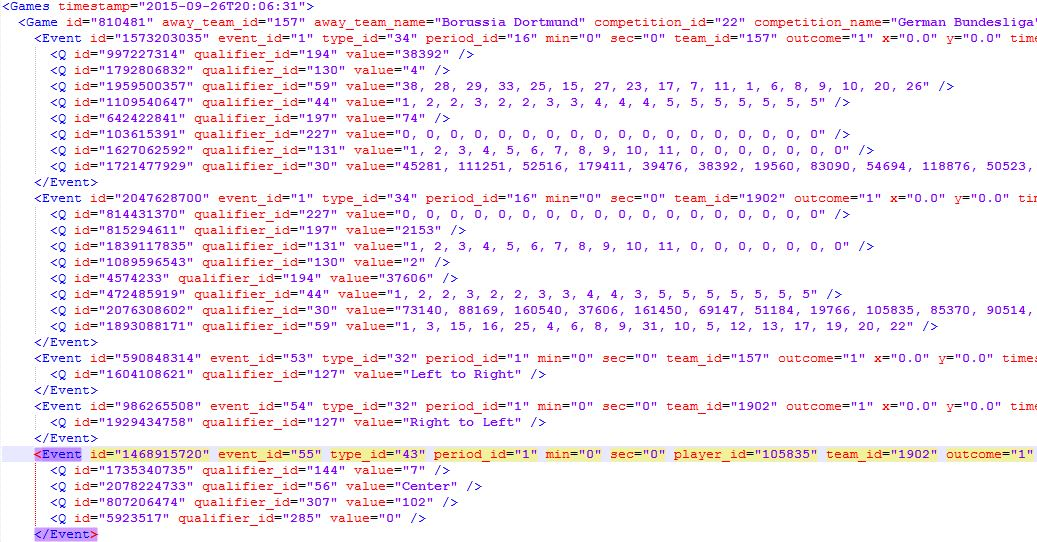
\includegraphics[scale=0.52]{se-wa-jpg/daten}
\caption{Auszug aus der XML-Datei mit den Events}
\label{xmldaten}
\end{figure}

Die \vref{xmldaten} zeigt einen Ausschnitt aus der XML-Datei in der alle Events eines Spiels aufzeichnet sind. Im oberen Teil sind die Mannschaftsaufstellungen zu sehen, wobei jeder Spieler eine eigene ID besitzt. Darunter folgt gelb markiert zum Anpfiff der Partie der erste Pass mit dem \textit{Outcome} 1, welcher einen erfolgreichen Pass identifiziert. 

\begin{sidewaysfigure}
\centering
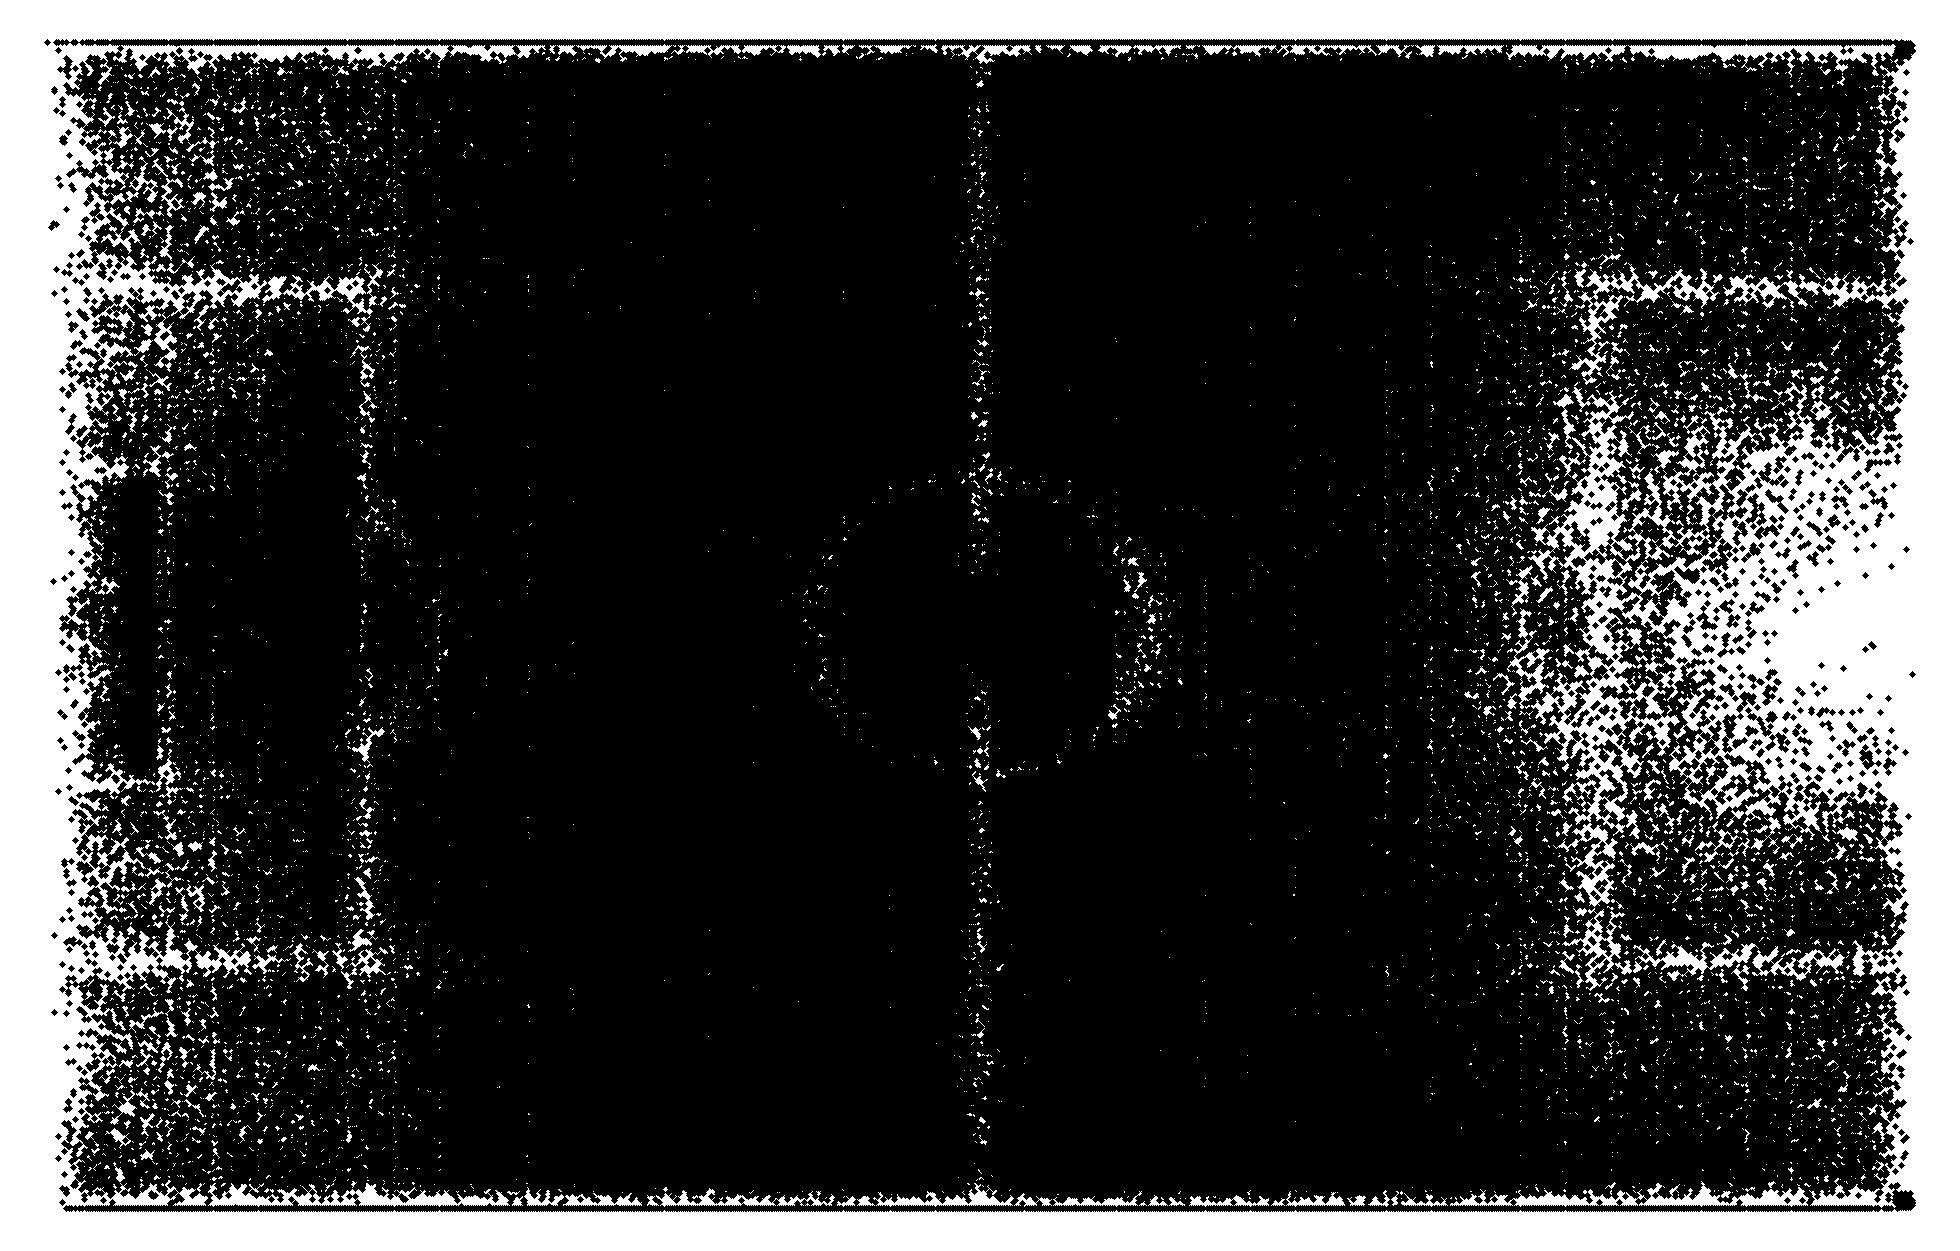
\includegraphics[scale=0.3]{se-wa-jpg/lines}
\caption[Problem der weißen Linien]{Problem der weißen Linien}
\label{lines}
\end{sidewaysfigure}

\chapter{MatLab}

\begin{figure}[H]
\centering
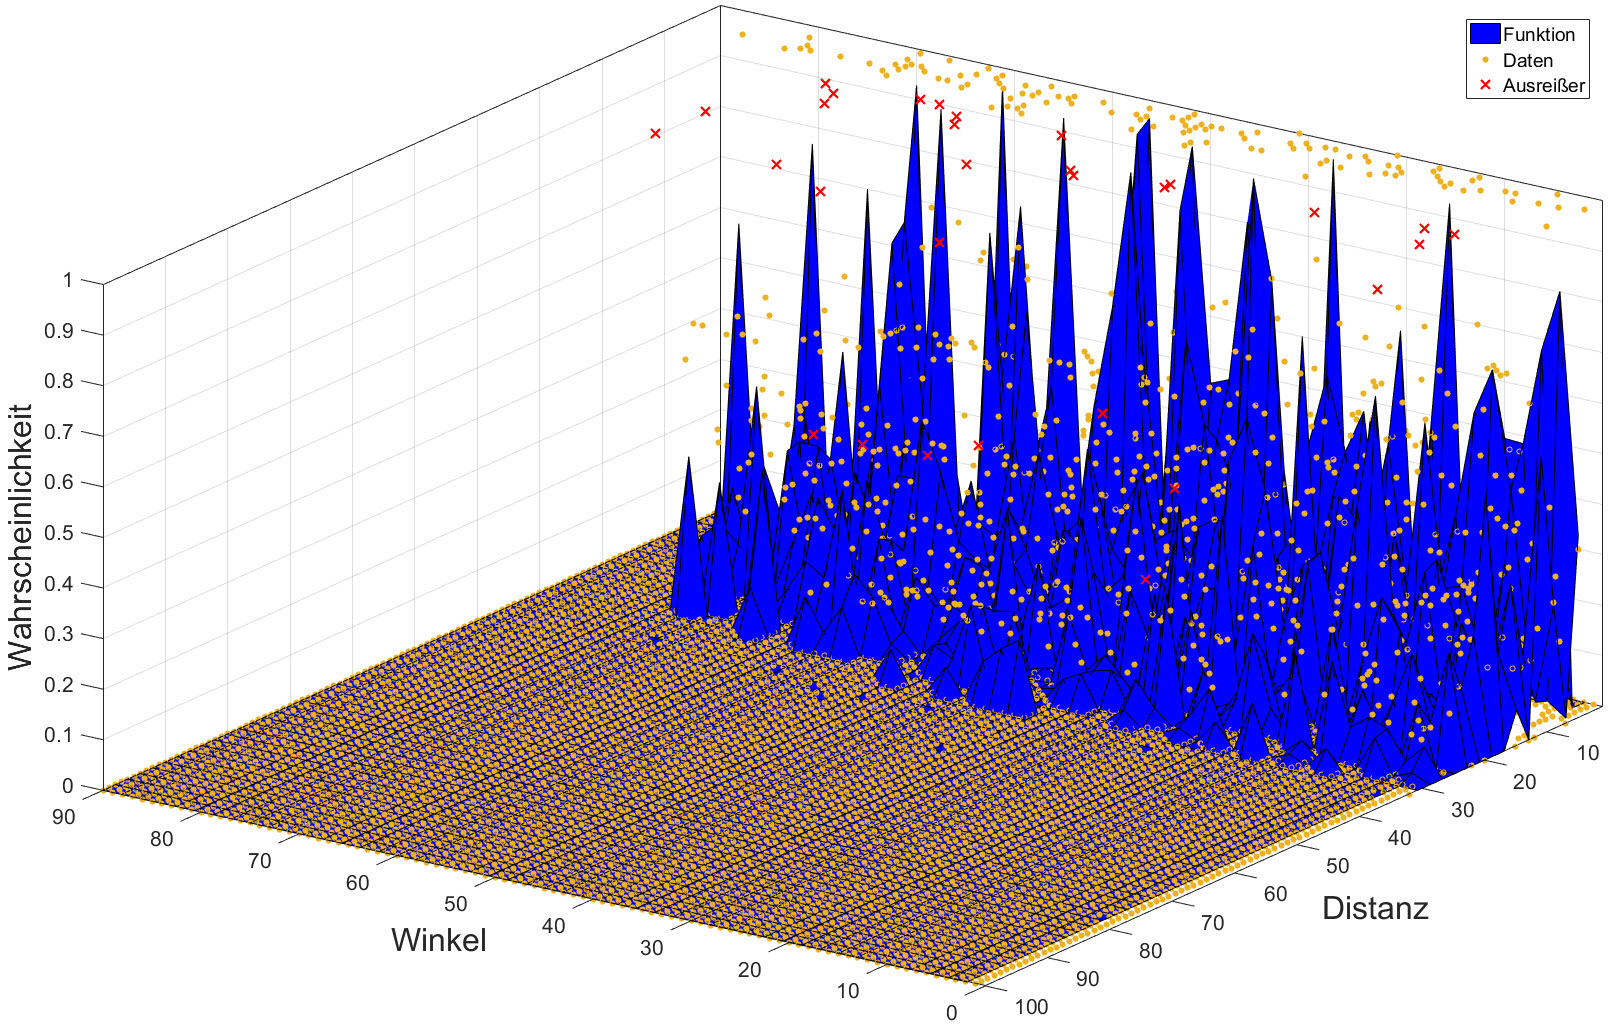
\includegraphics[scale=0.34]{se-wa-jpg/inter}
\caption{Ausschluss der Interpolation}
\label{inter}
\end{figure}

\begin{figure}[H]
\centering
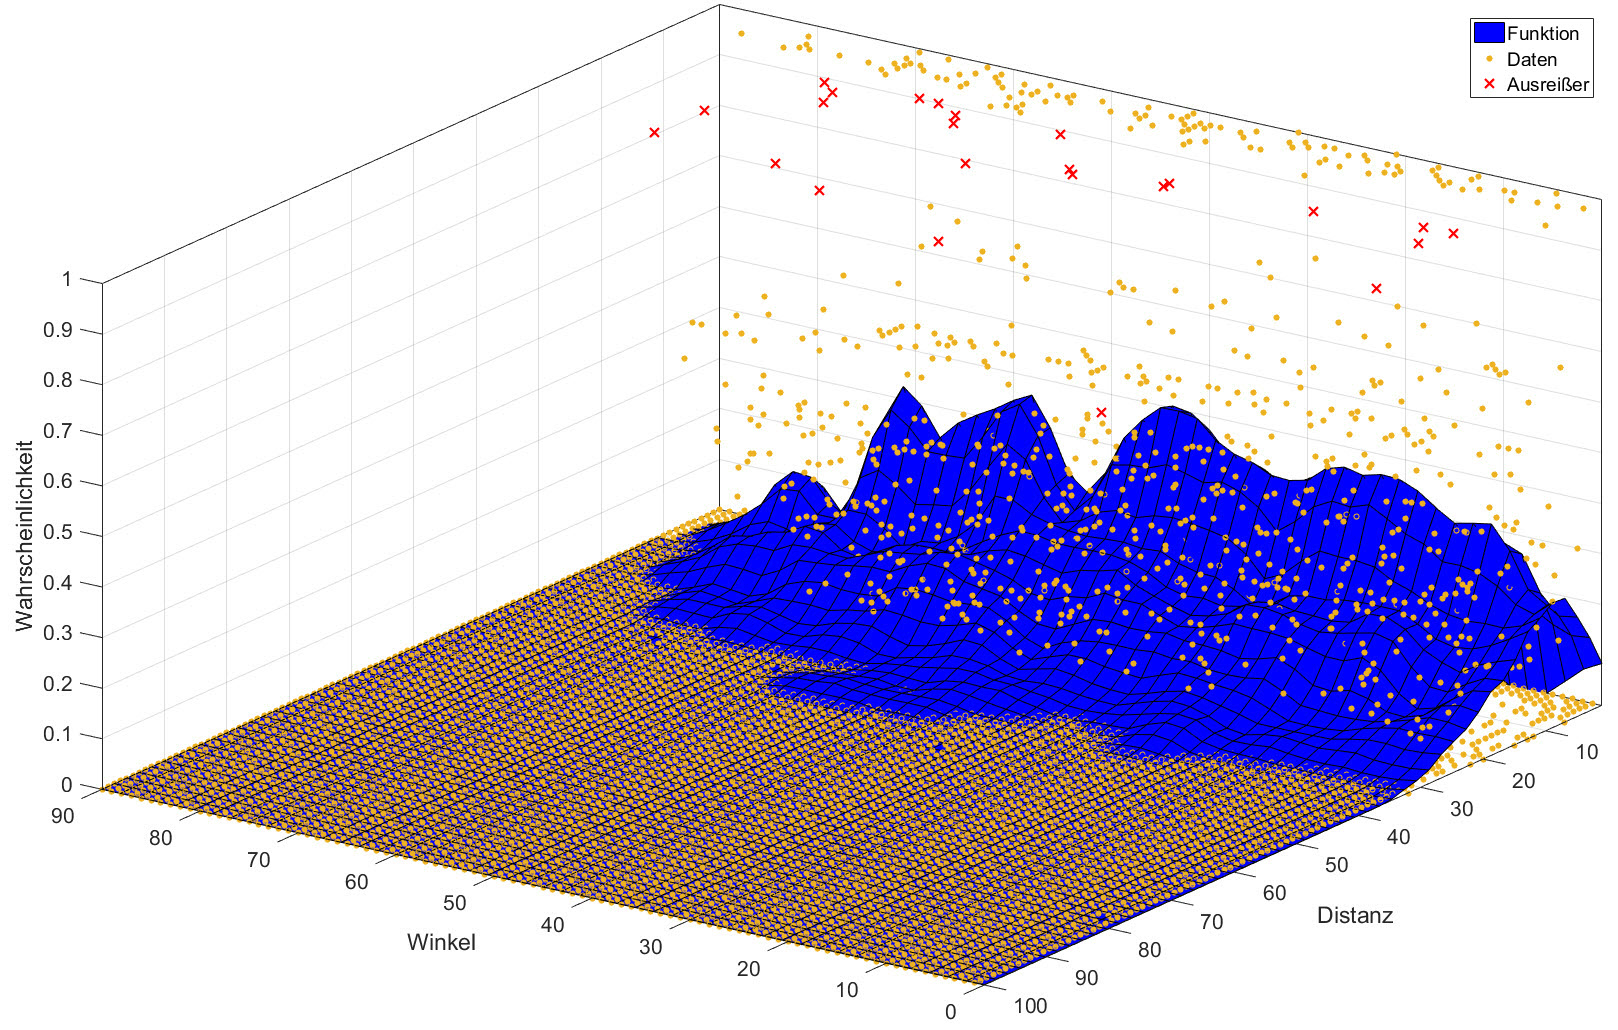
\includegraphics[scale=0.34]{se-wa-jpg/splinewdTM}
\caption{Overfitting bei einem Span-Wert von 1\%}
\label{splinewdTM}
\end{figure}

\begin{figure}[H]
\centering
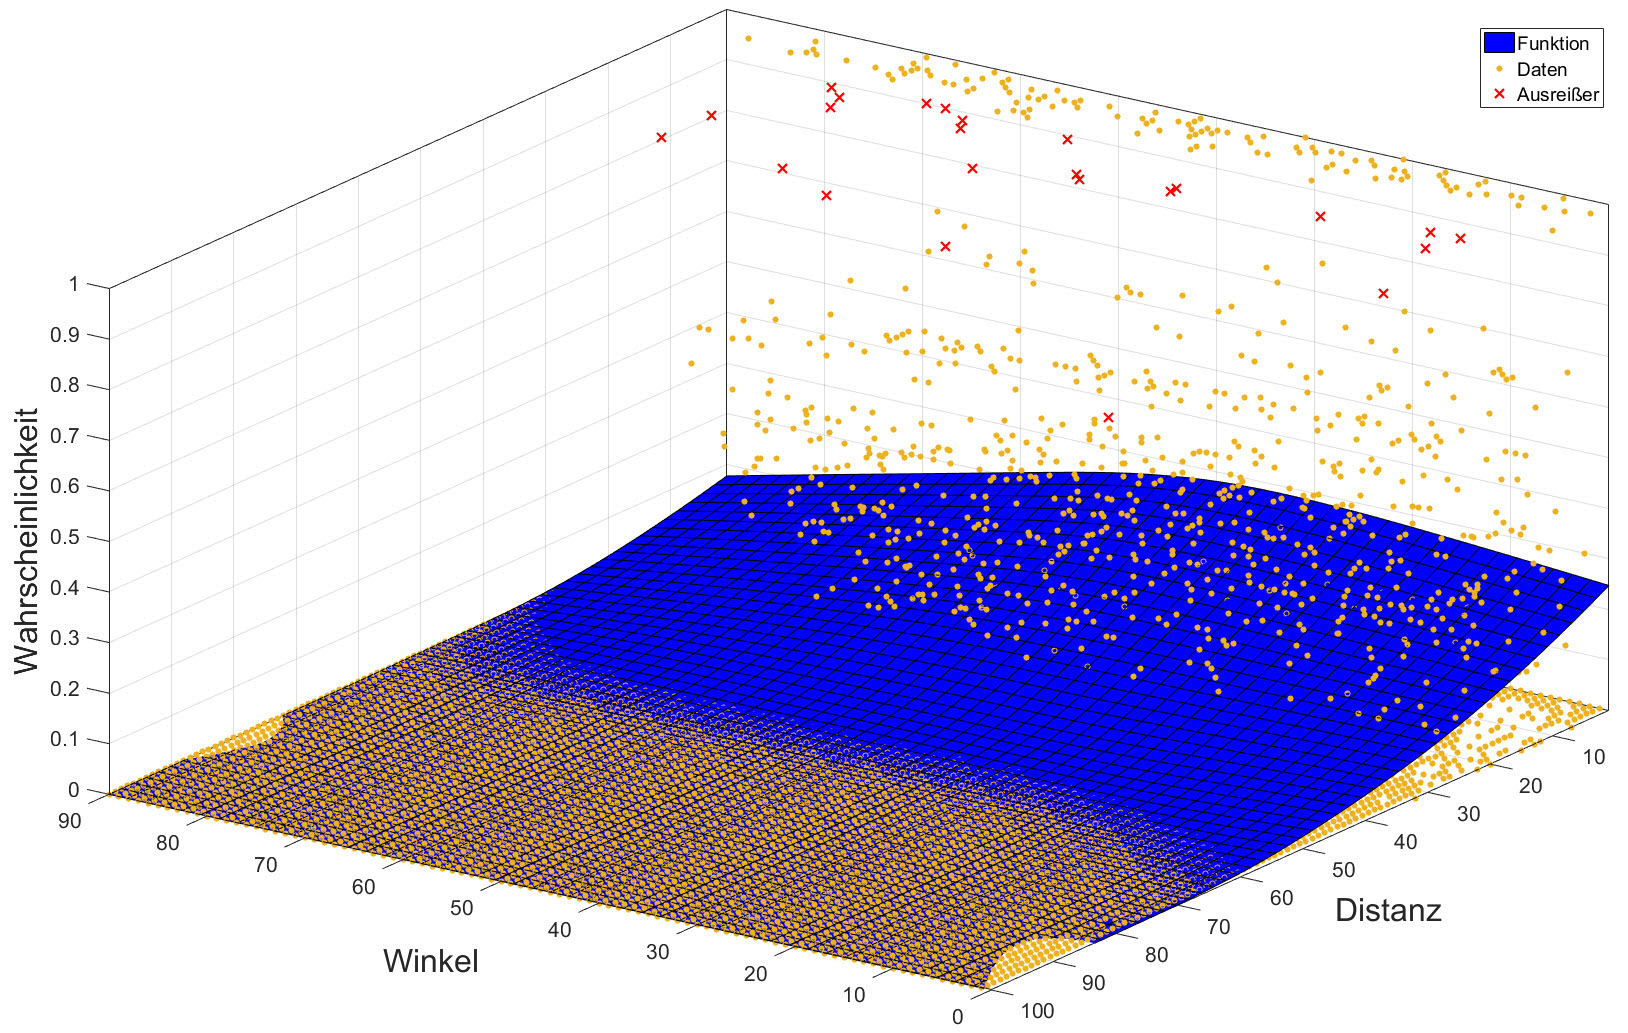
\includegraphics[scale=0.34]{se-wa-jpg/splinewdTL}
\caption{Underfitting bei einem Span-Wert von 50\%}
\label{splinewdTL}
\end{figure}

\chapter{Evaluation}
\label{anheva}

Hier werden die Ergebnisse der Evaluation des nichtparametrischen Regressionsmodelles unter der Betrachtung der Position des Schusses dokumentiert. 

\begin{sidewaysfigure}
\centering
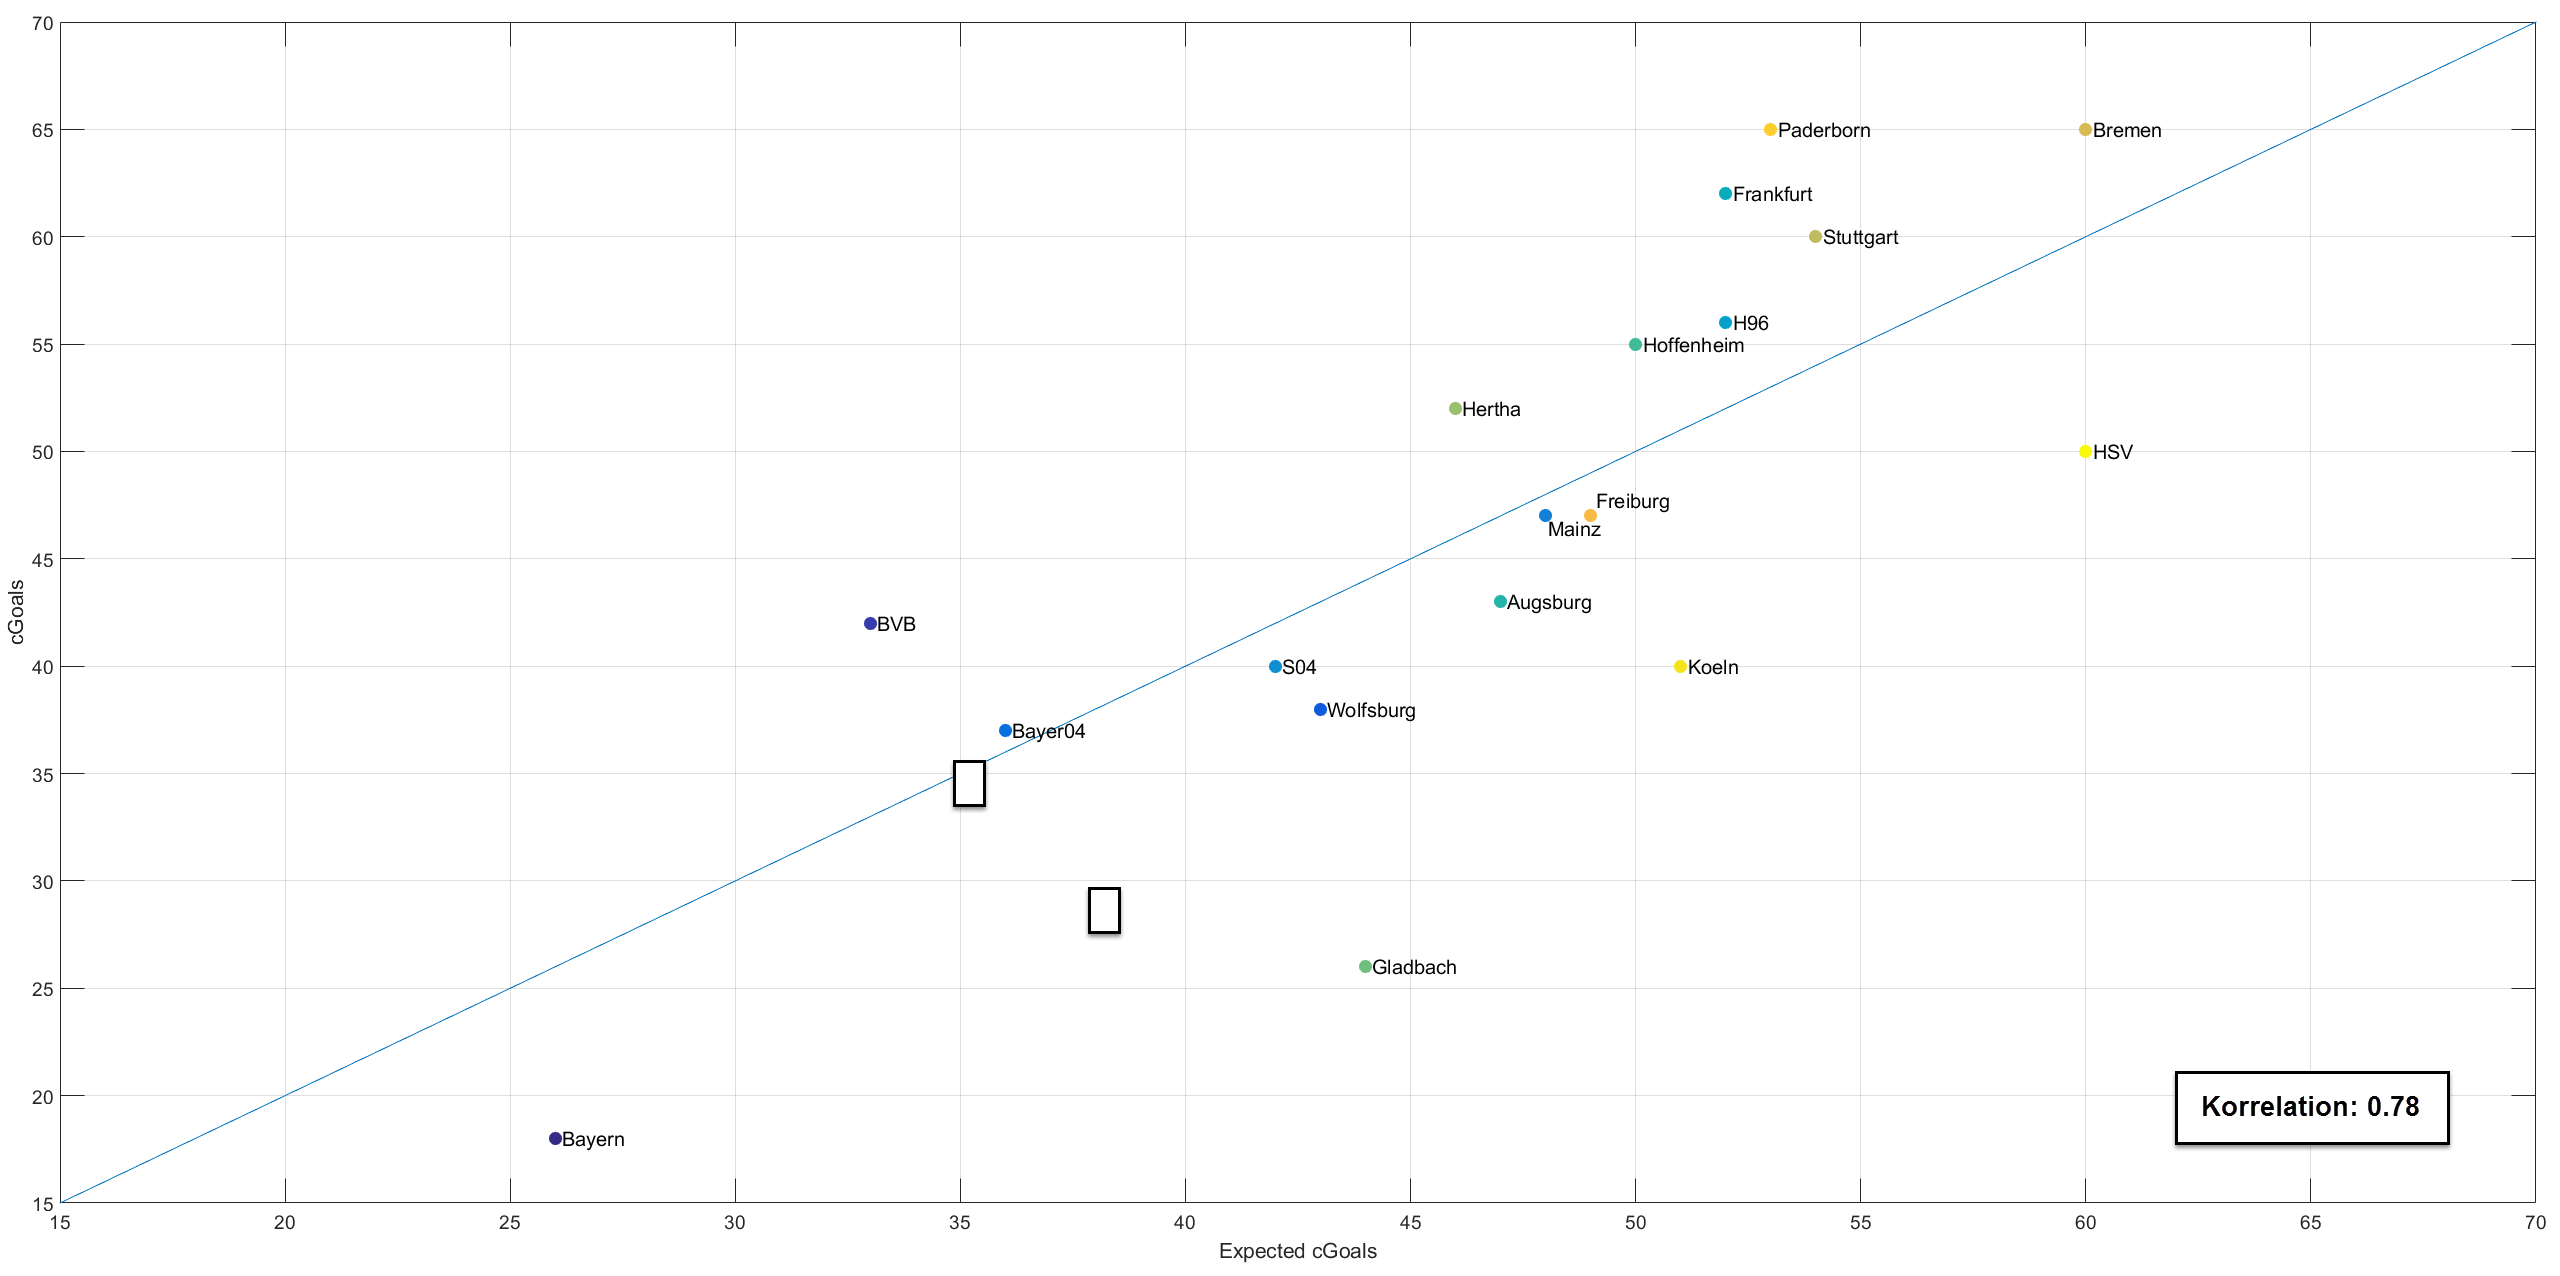
\includegraphics[scale=0.3]{se-wa-jpg/cGoals_correlation_14_15}
\caption{Evaluation der Gegentore der Saison 2014/15}
\label{cg1415}
\end{sidewaysfigure}

\begin{sidewaysfigure}
\centering
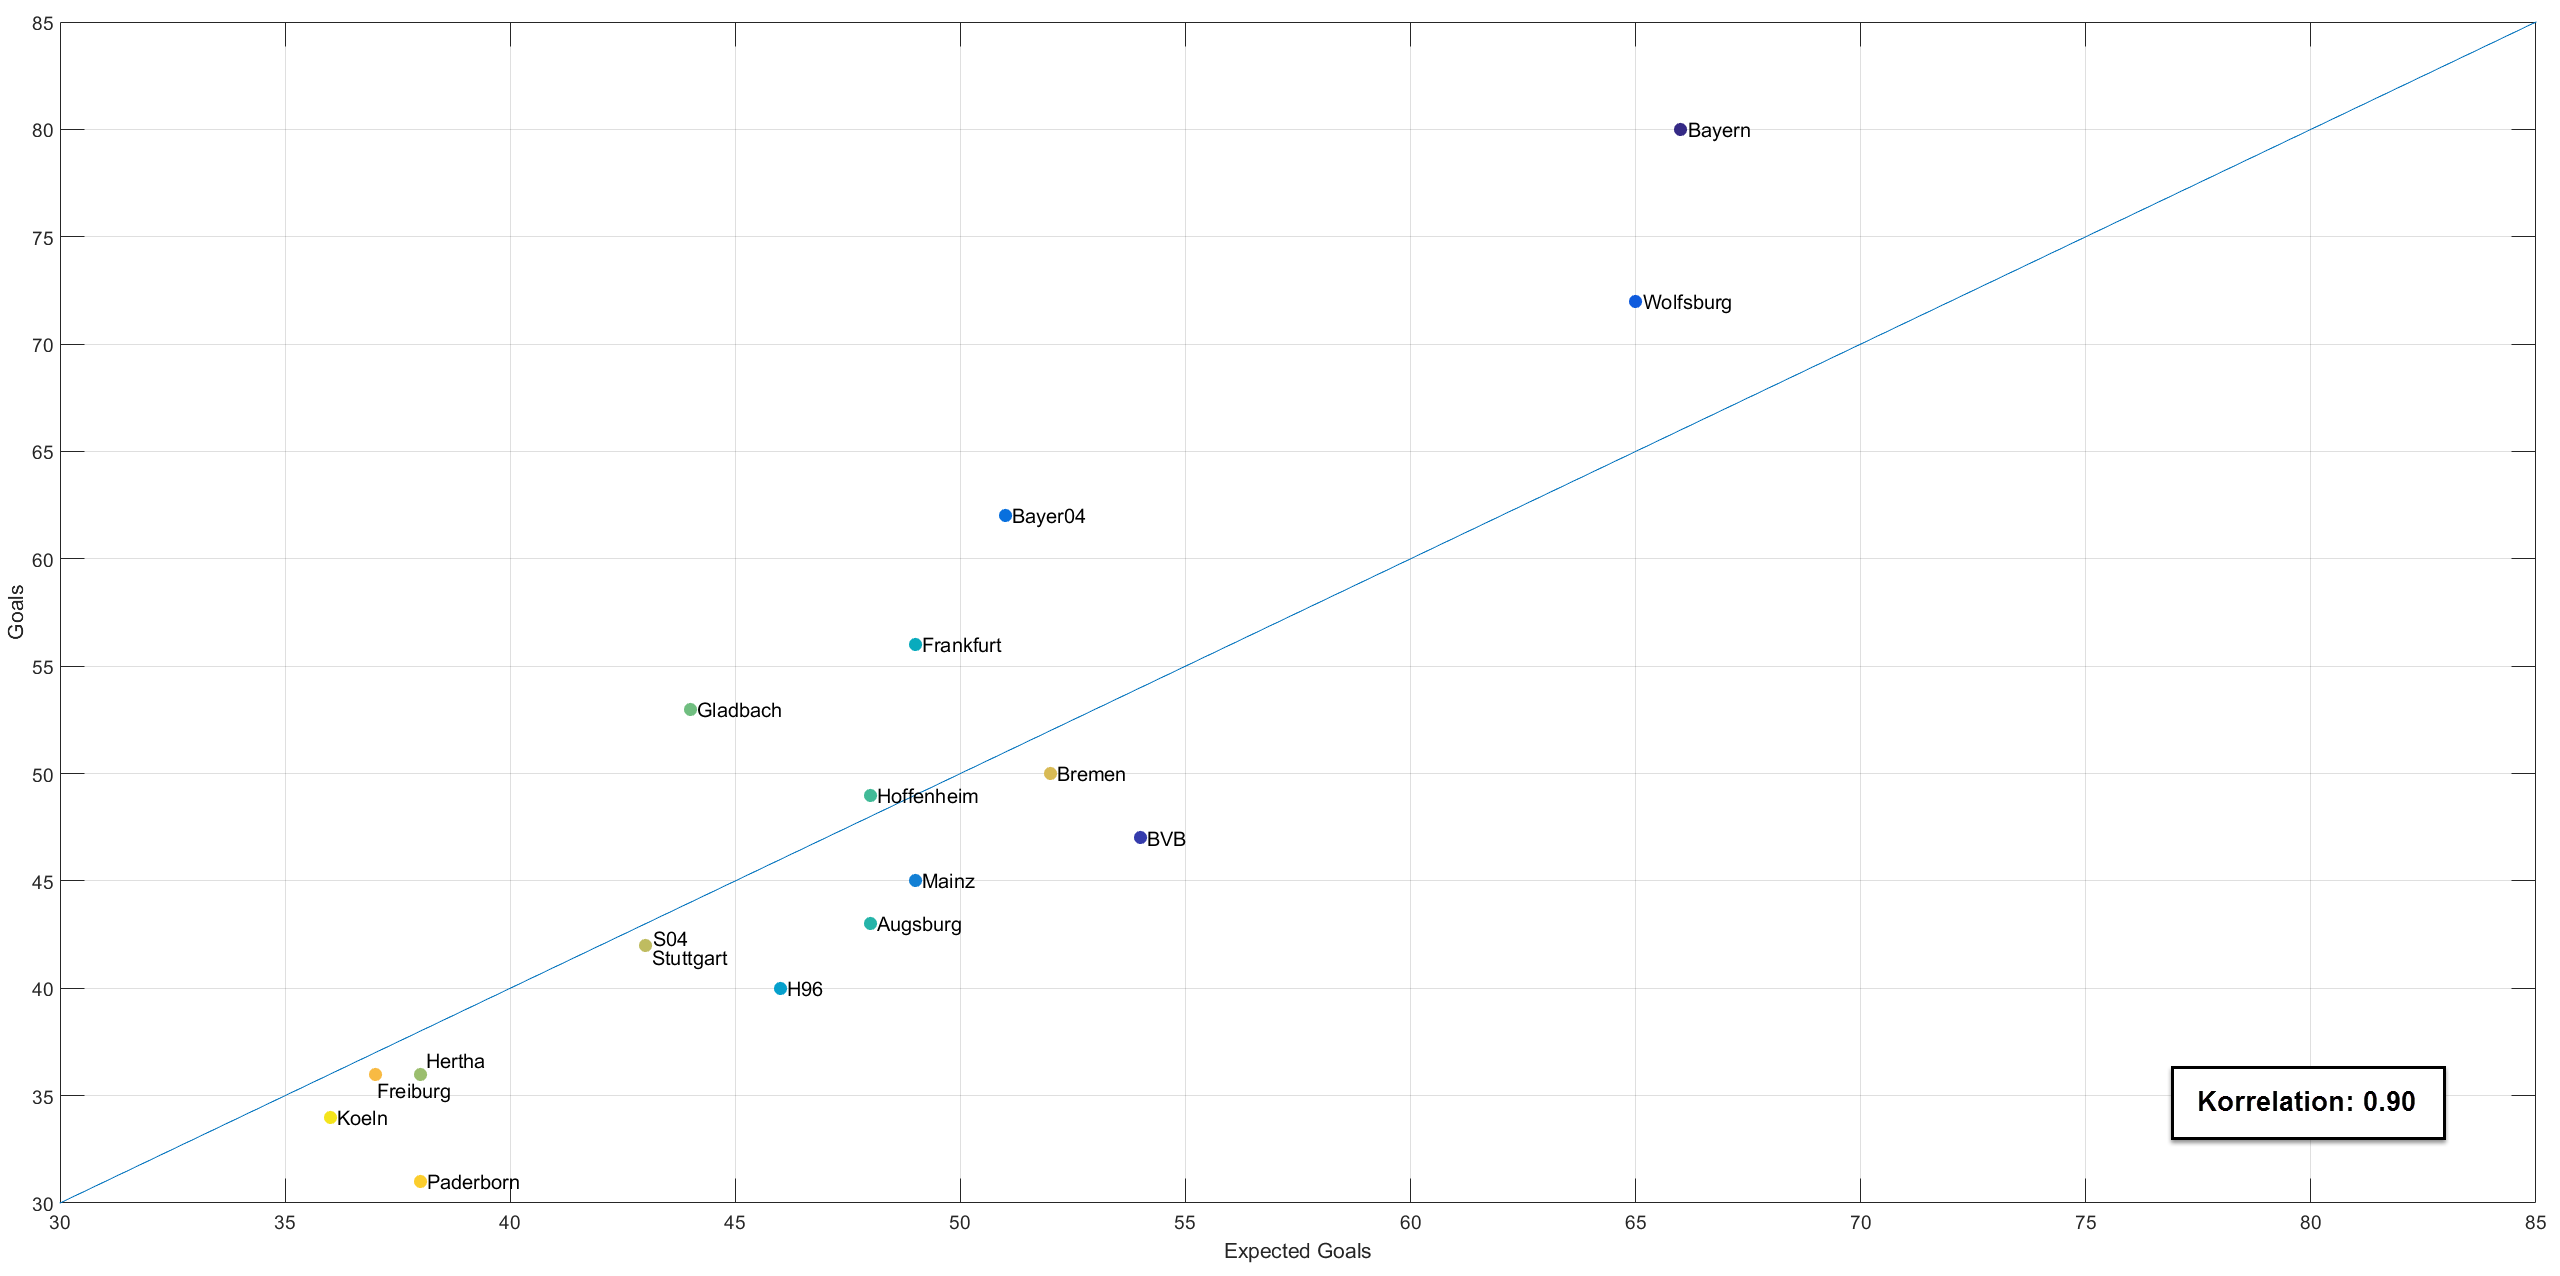
\includegraphics[scale=0.3]{se-wa-jpg/goals_correlation_14_15}
\caption{Evaluation der Tore der Saison 2014/15}
\label{g1415}
\end{sidewaysfigure}

\begin{sidewaysfigure}
\centering
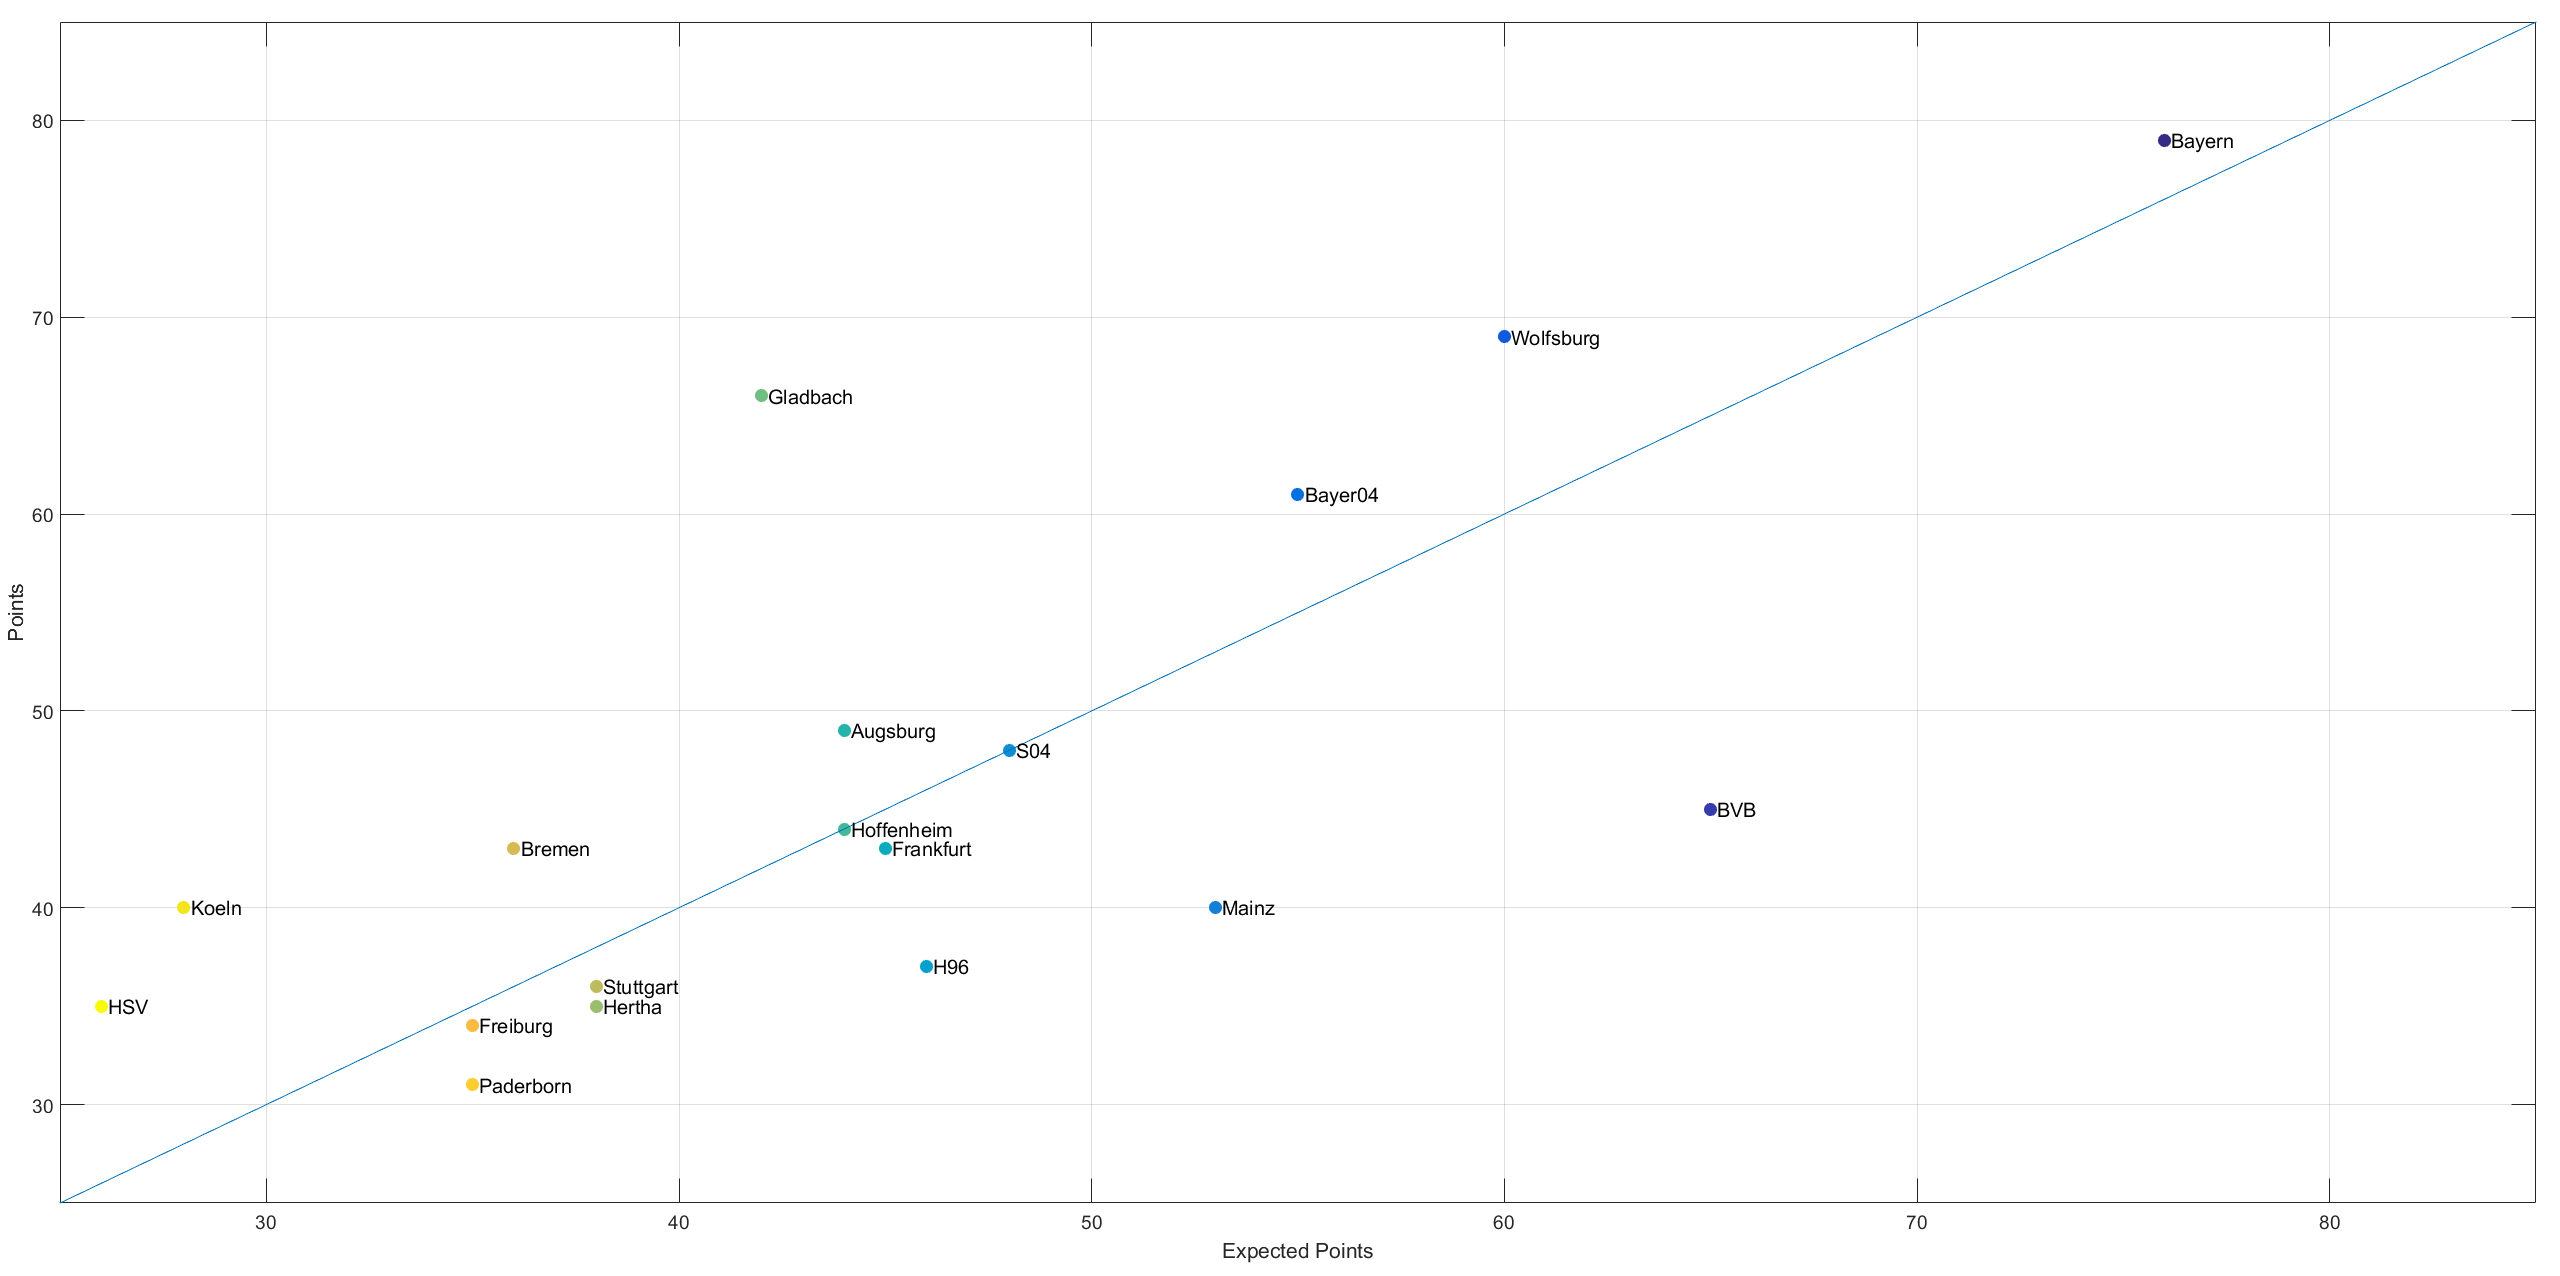
\includegraphics[scale=0.3]{se-wa-jpg/points_correlation_14_15}
\caption{Evaluation der Punkte der Saison 2014/15}
\label{p1415}
\end{sidewaysfigure}

\begin{sidewaysfigure}
\centering
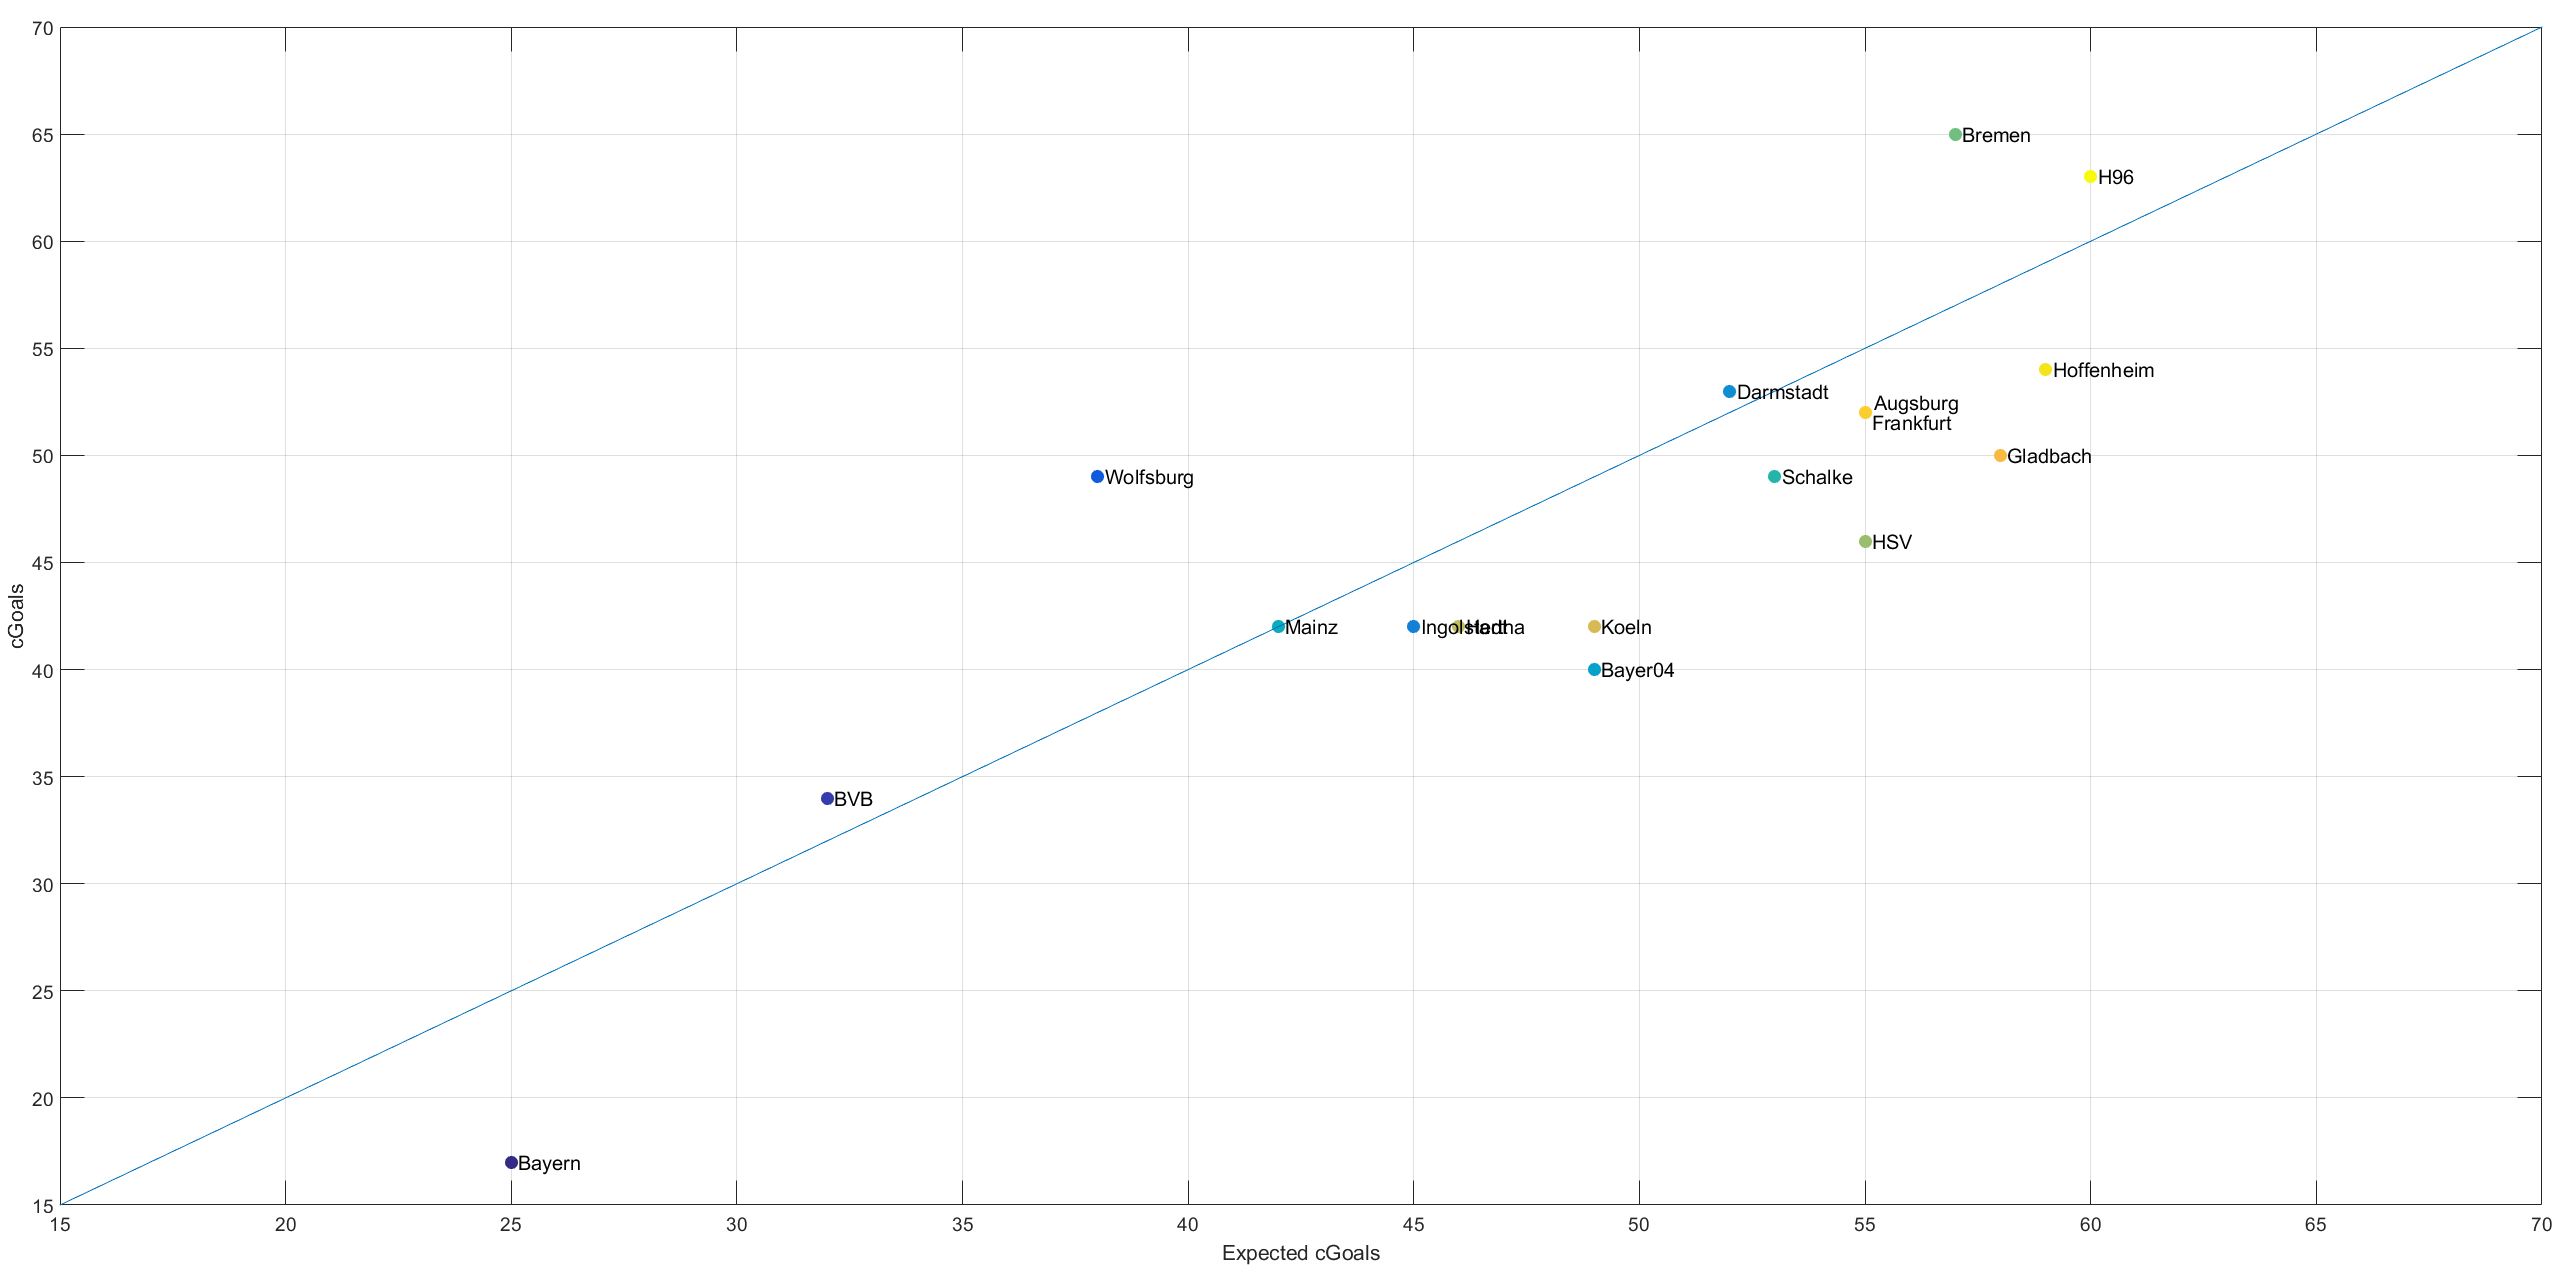
\includegraphics[scale=0.3]{se-wa-jpg/cGoals_correlation_15_16}
\caption{Evaluation der Gegentore der Saison 2015/16}
\label{lines}
\end{sidewaysfigure}

\begin{sidewaysfigure}
\centering
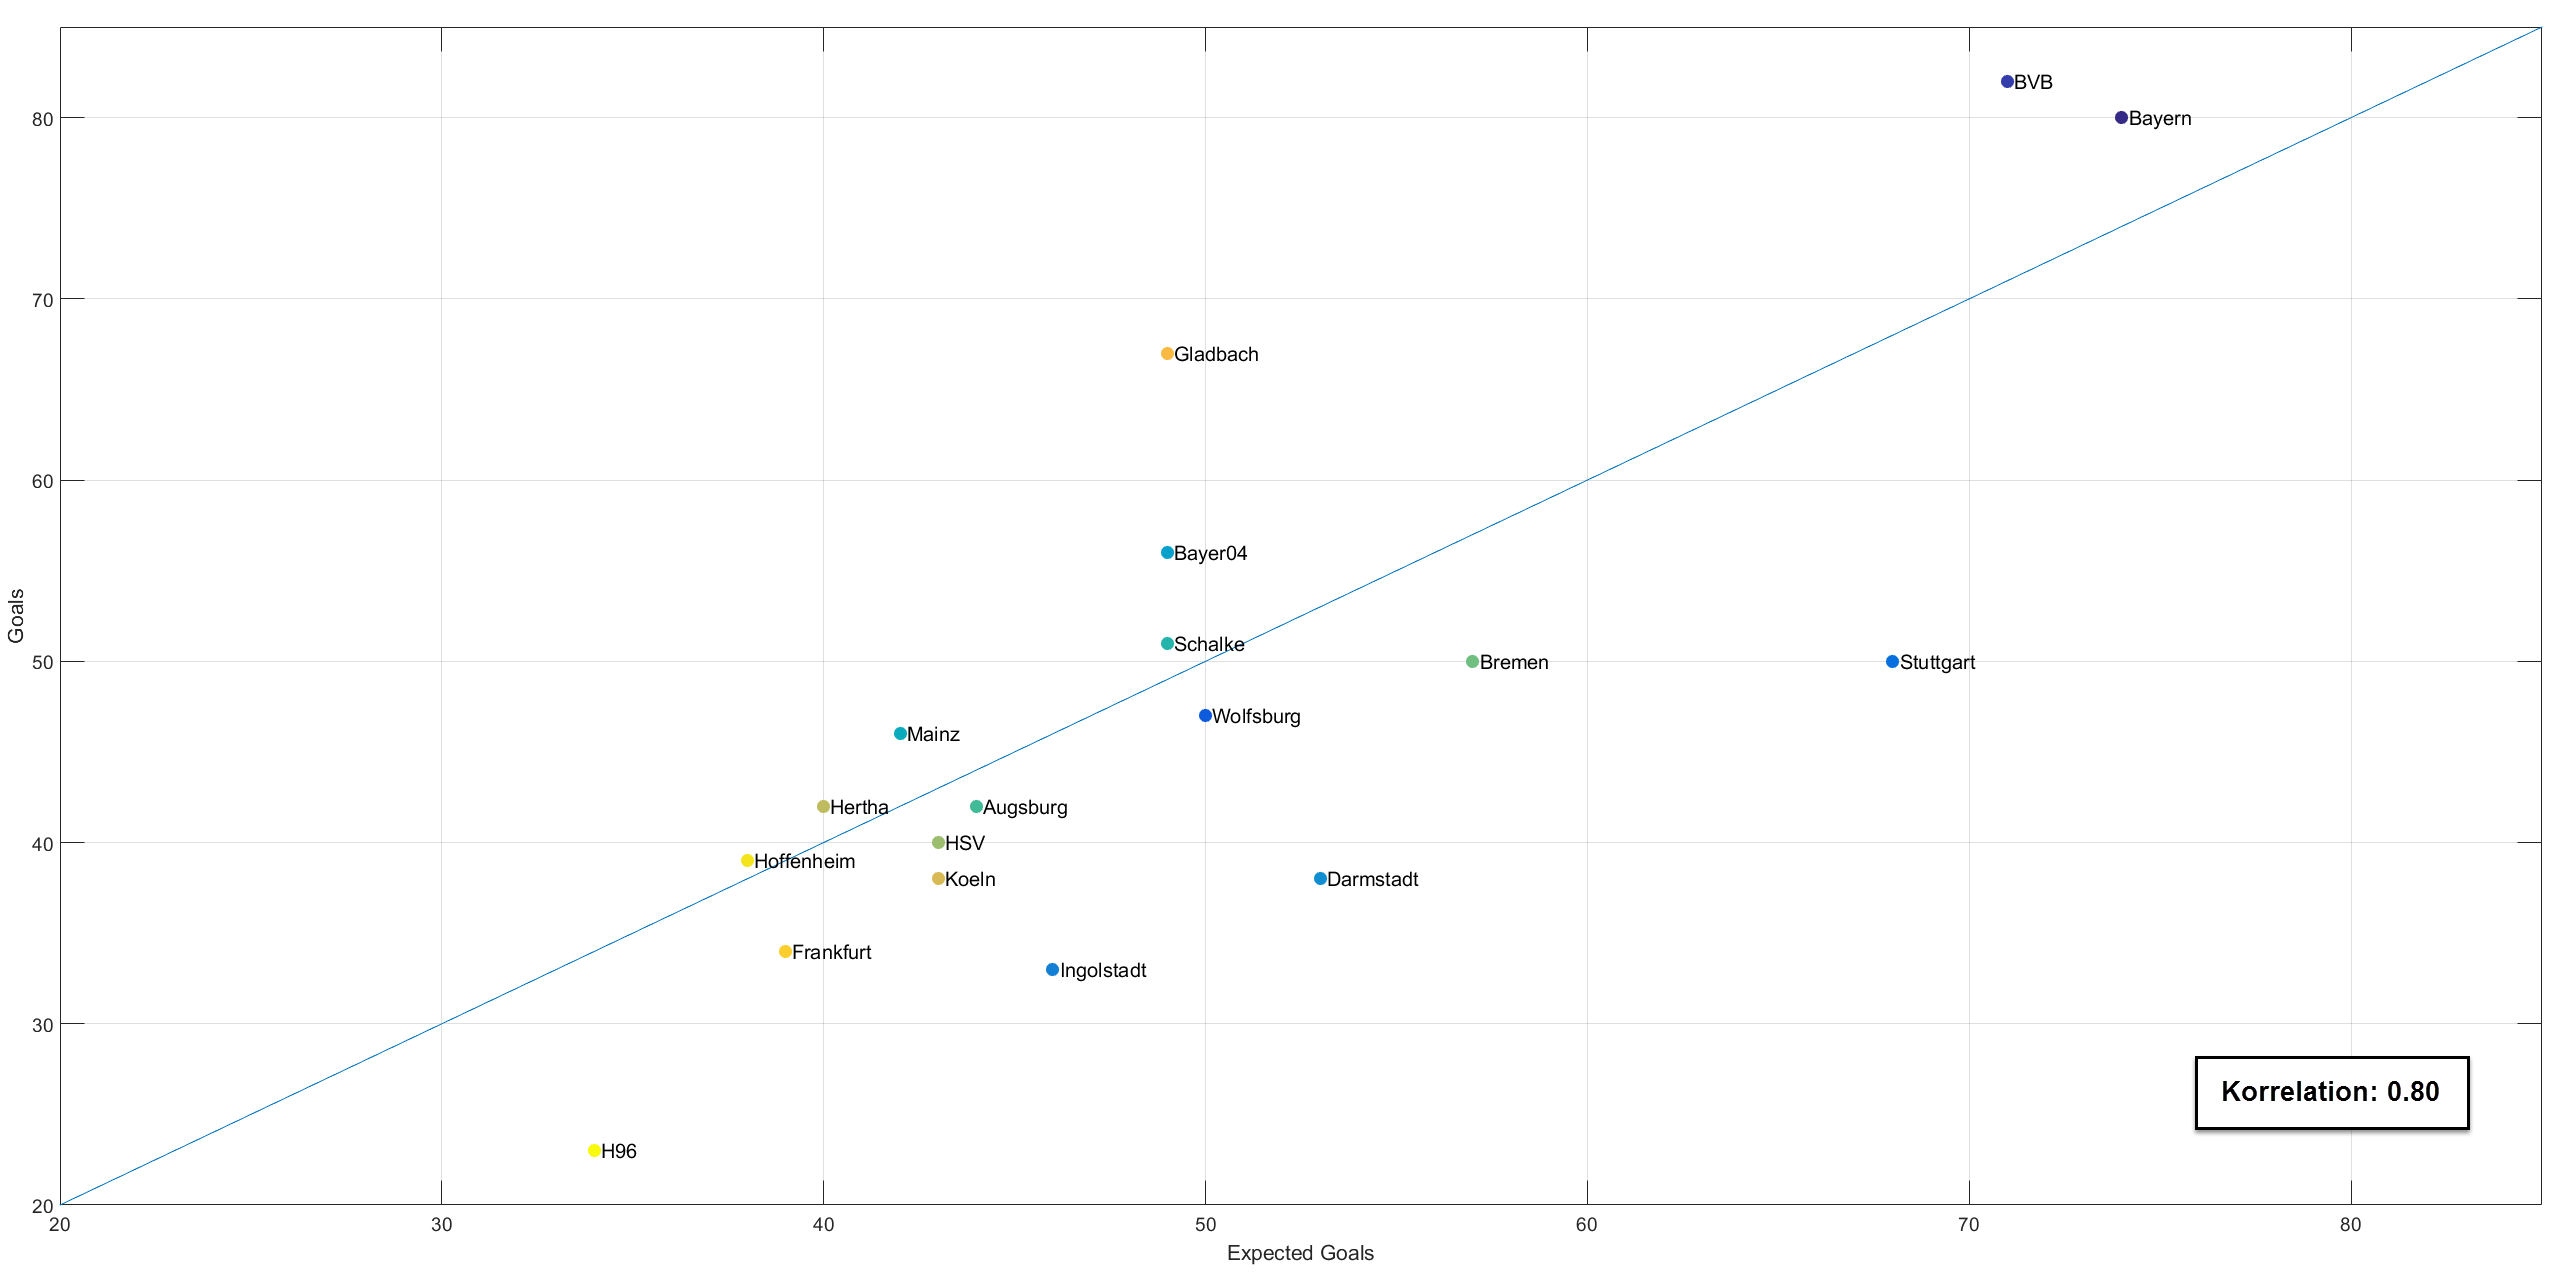
\includegraphics[scale=0.3]{se-wa-jpg/goals_correlation_15_16}
\caption{Evaluation der Tore der Saison 2015/16}
\label{lines}
\end{sidewaysfigure}

\begin{sidewaysfigure}
\centering
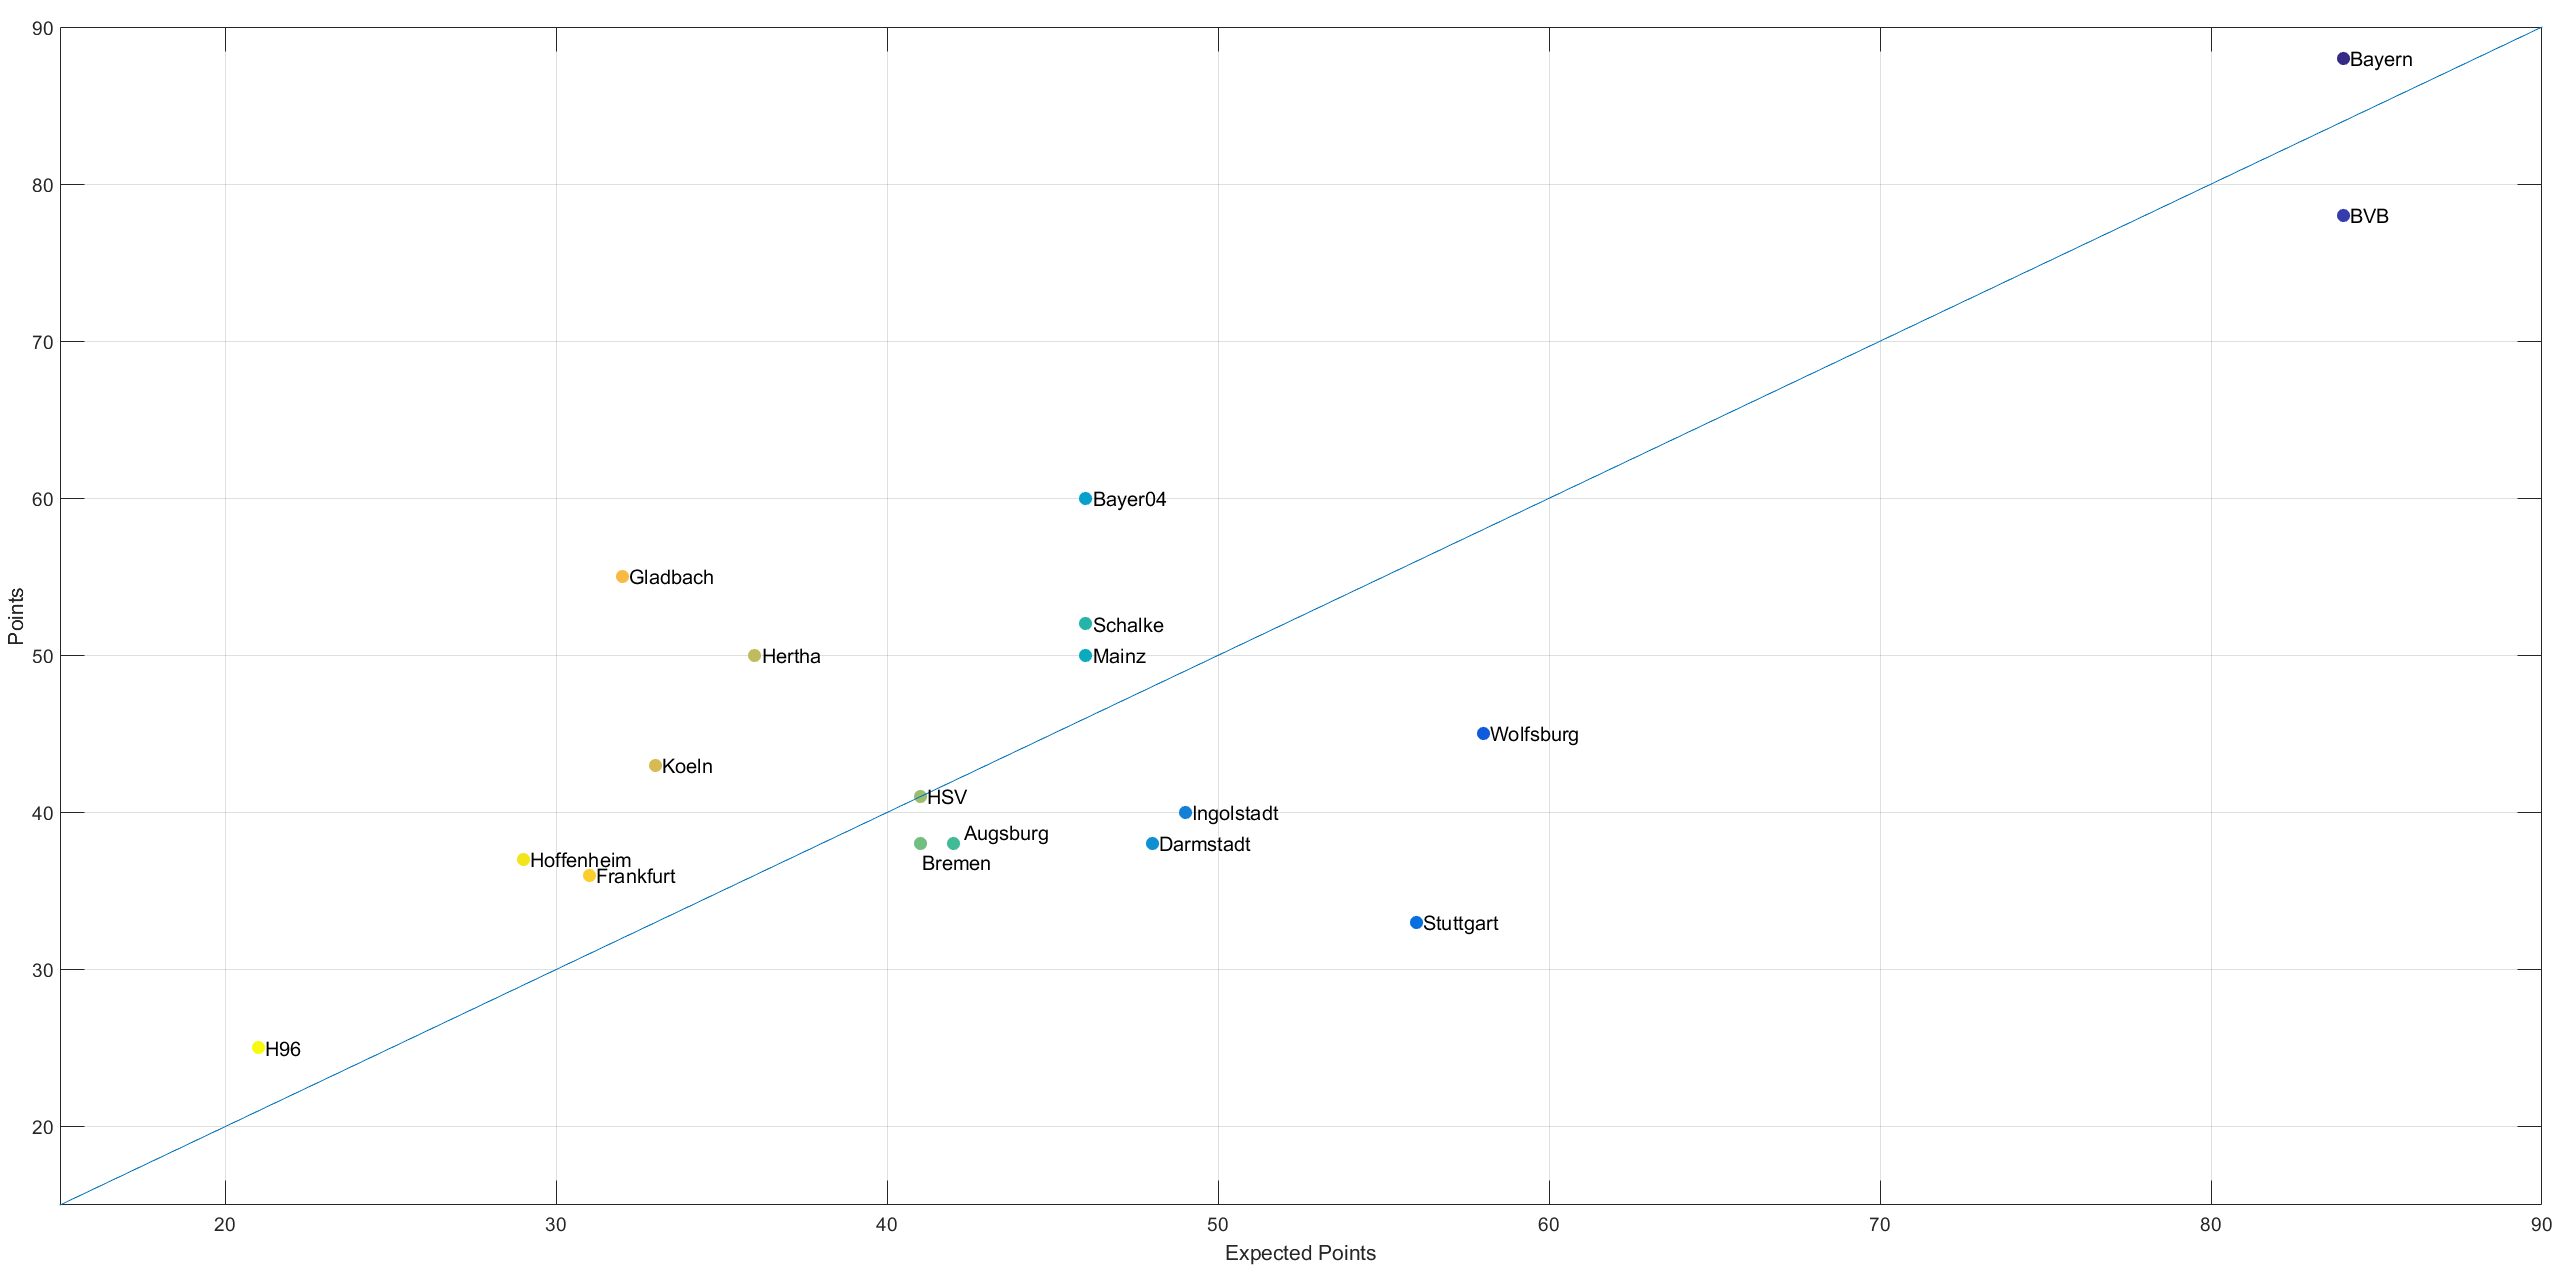
\includegraphics[scale=0.3]{se-wa-jpg/points_correlation_15_16}
\caption{Evaluation der Punkte der Saison 2015/16}
\label{lines}
\end{sidewaysfigure}

\begin{sidewaysfigure}
\centering
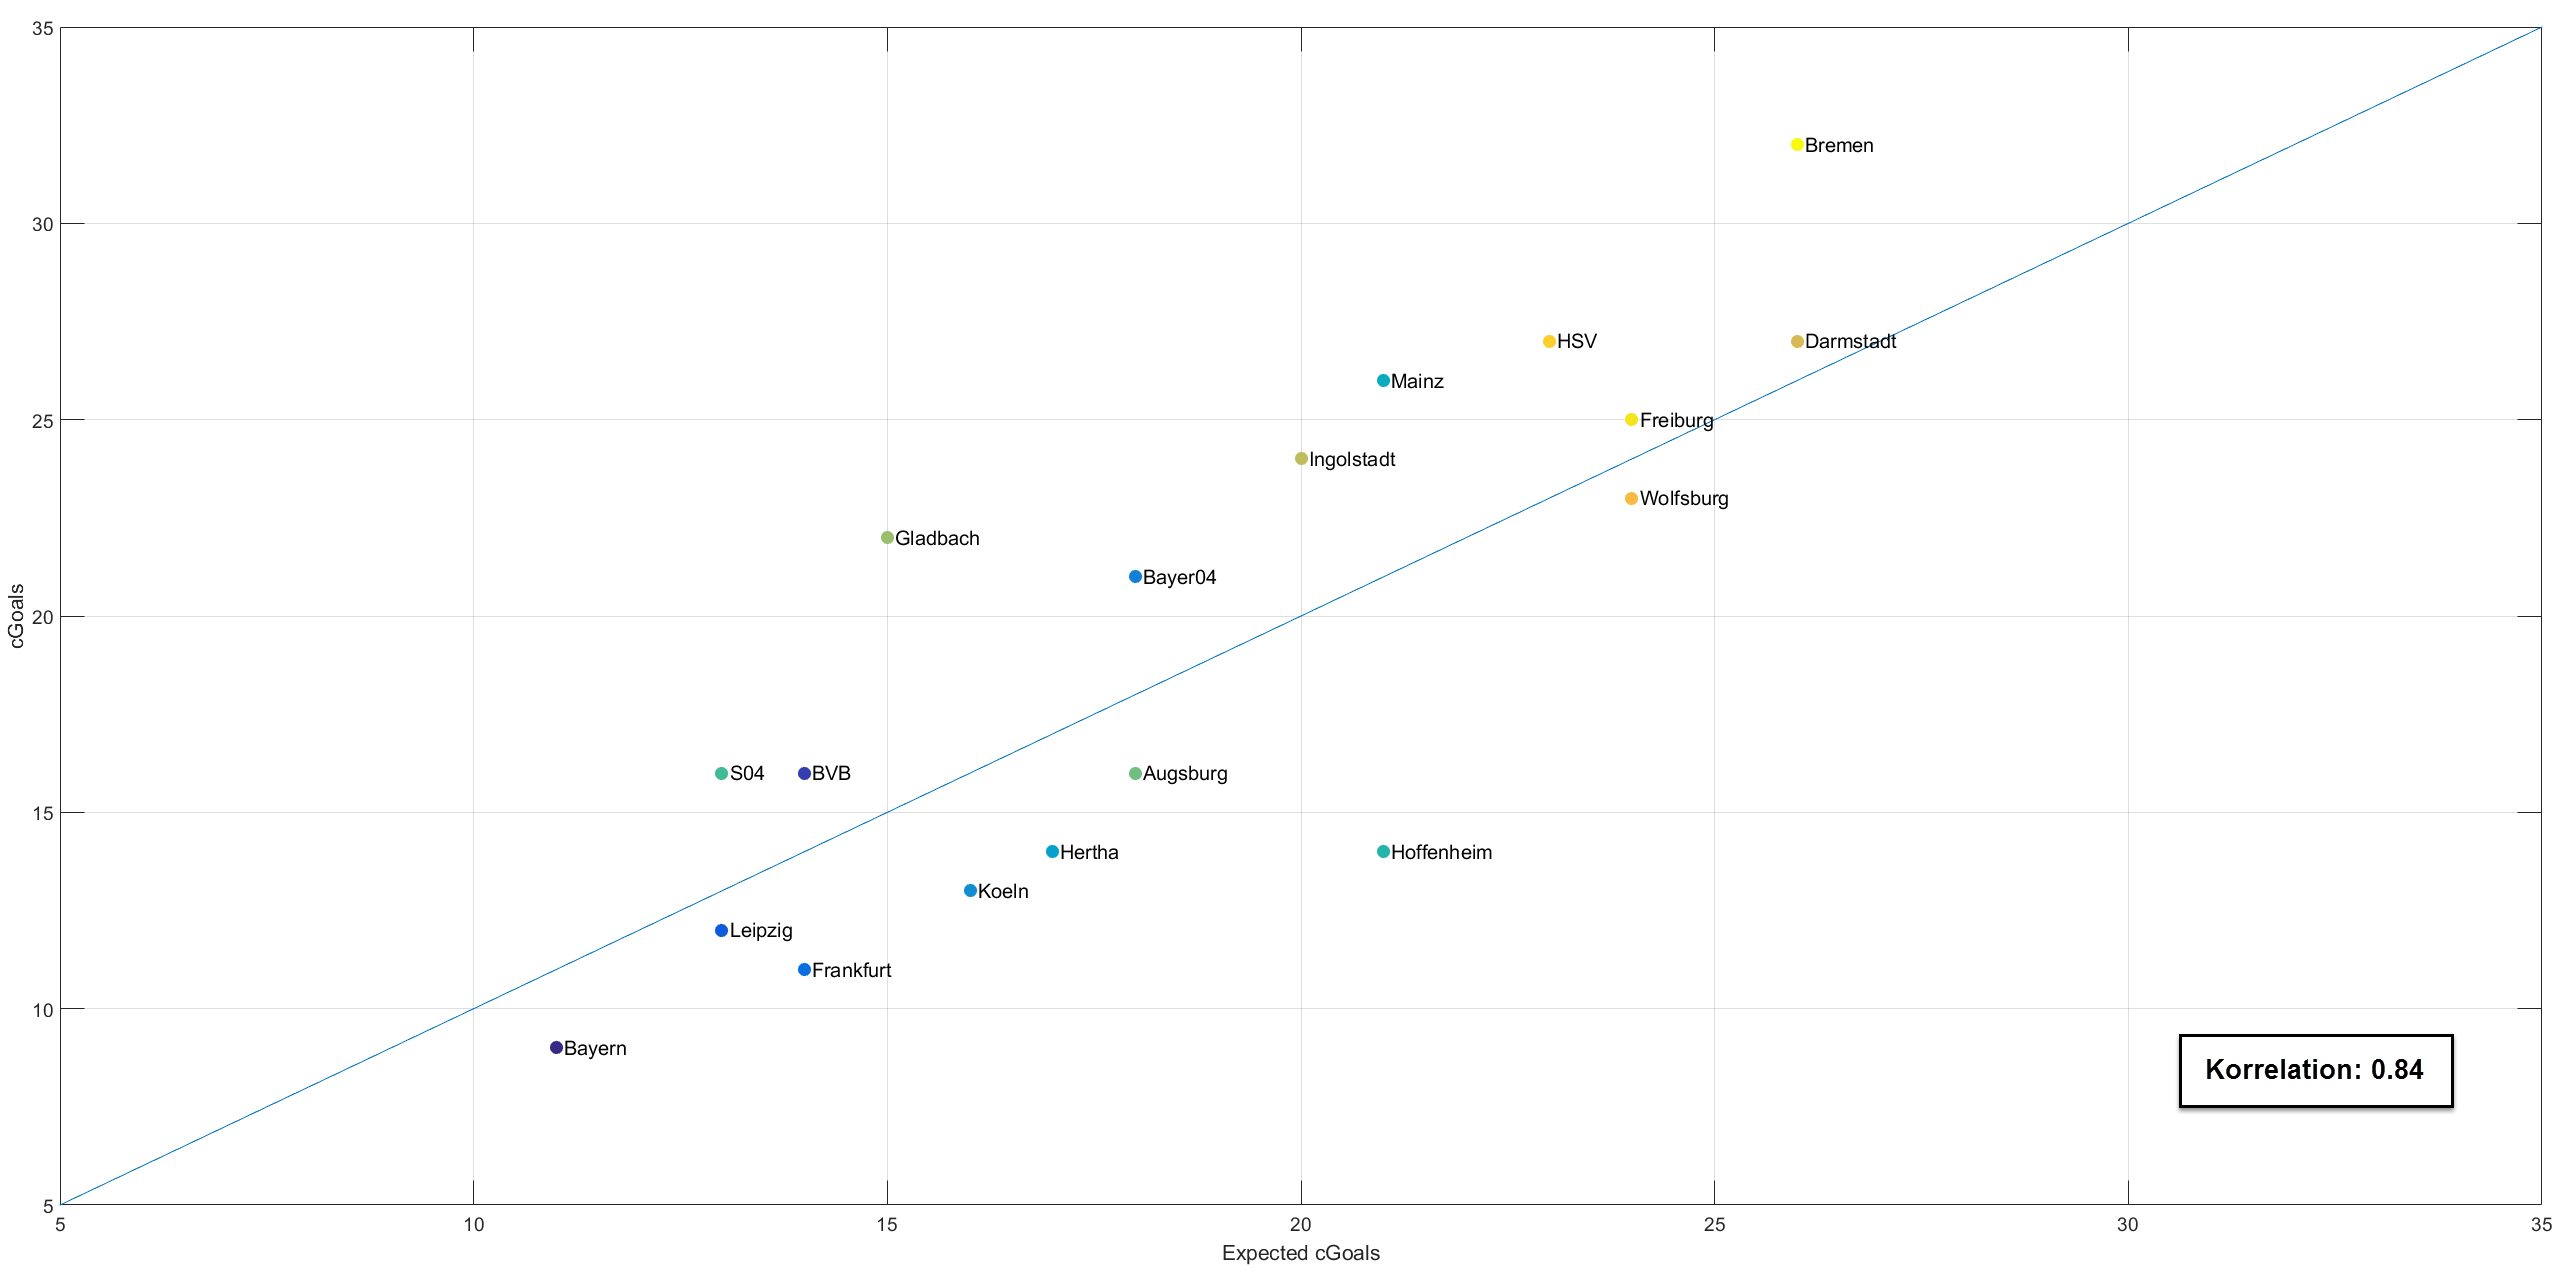
\includegraphics[scale=0.3]{se-wa-jpg/cGoals_correlation_16_17}
\caption{Evaluation der Gegentore der Saison 2016/17}
\label{lines}
\end{sidewaysfigure}

\begin{sidewaysfigure}
\centering
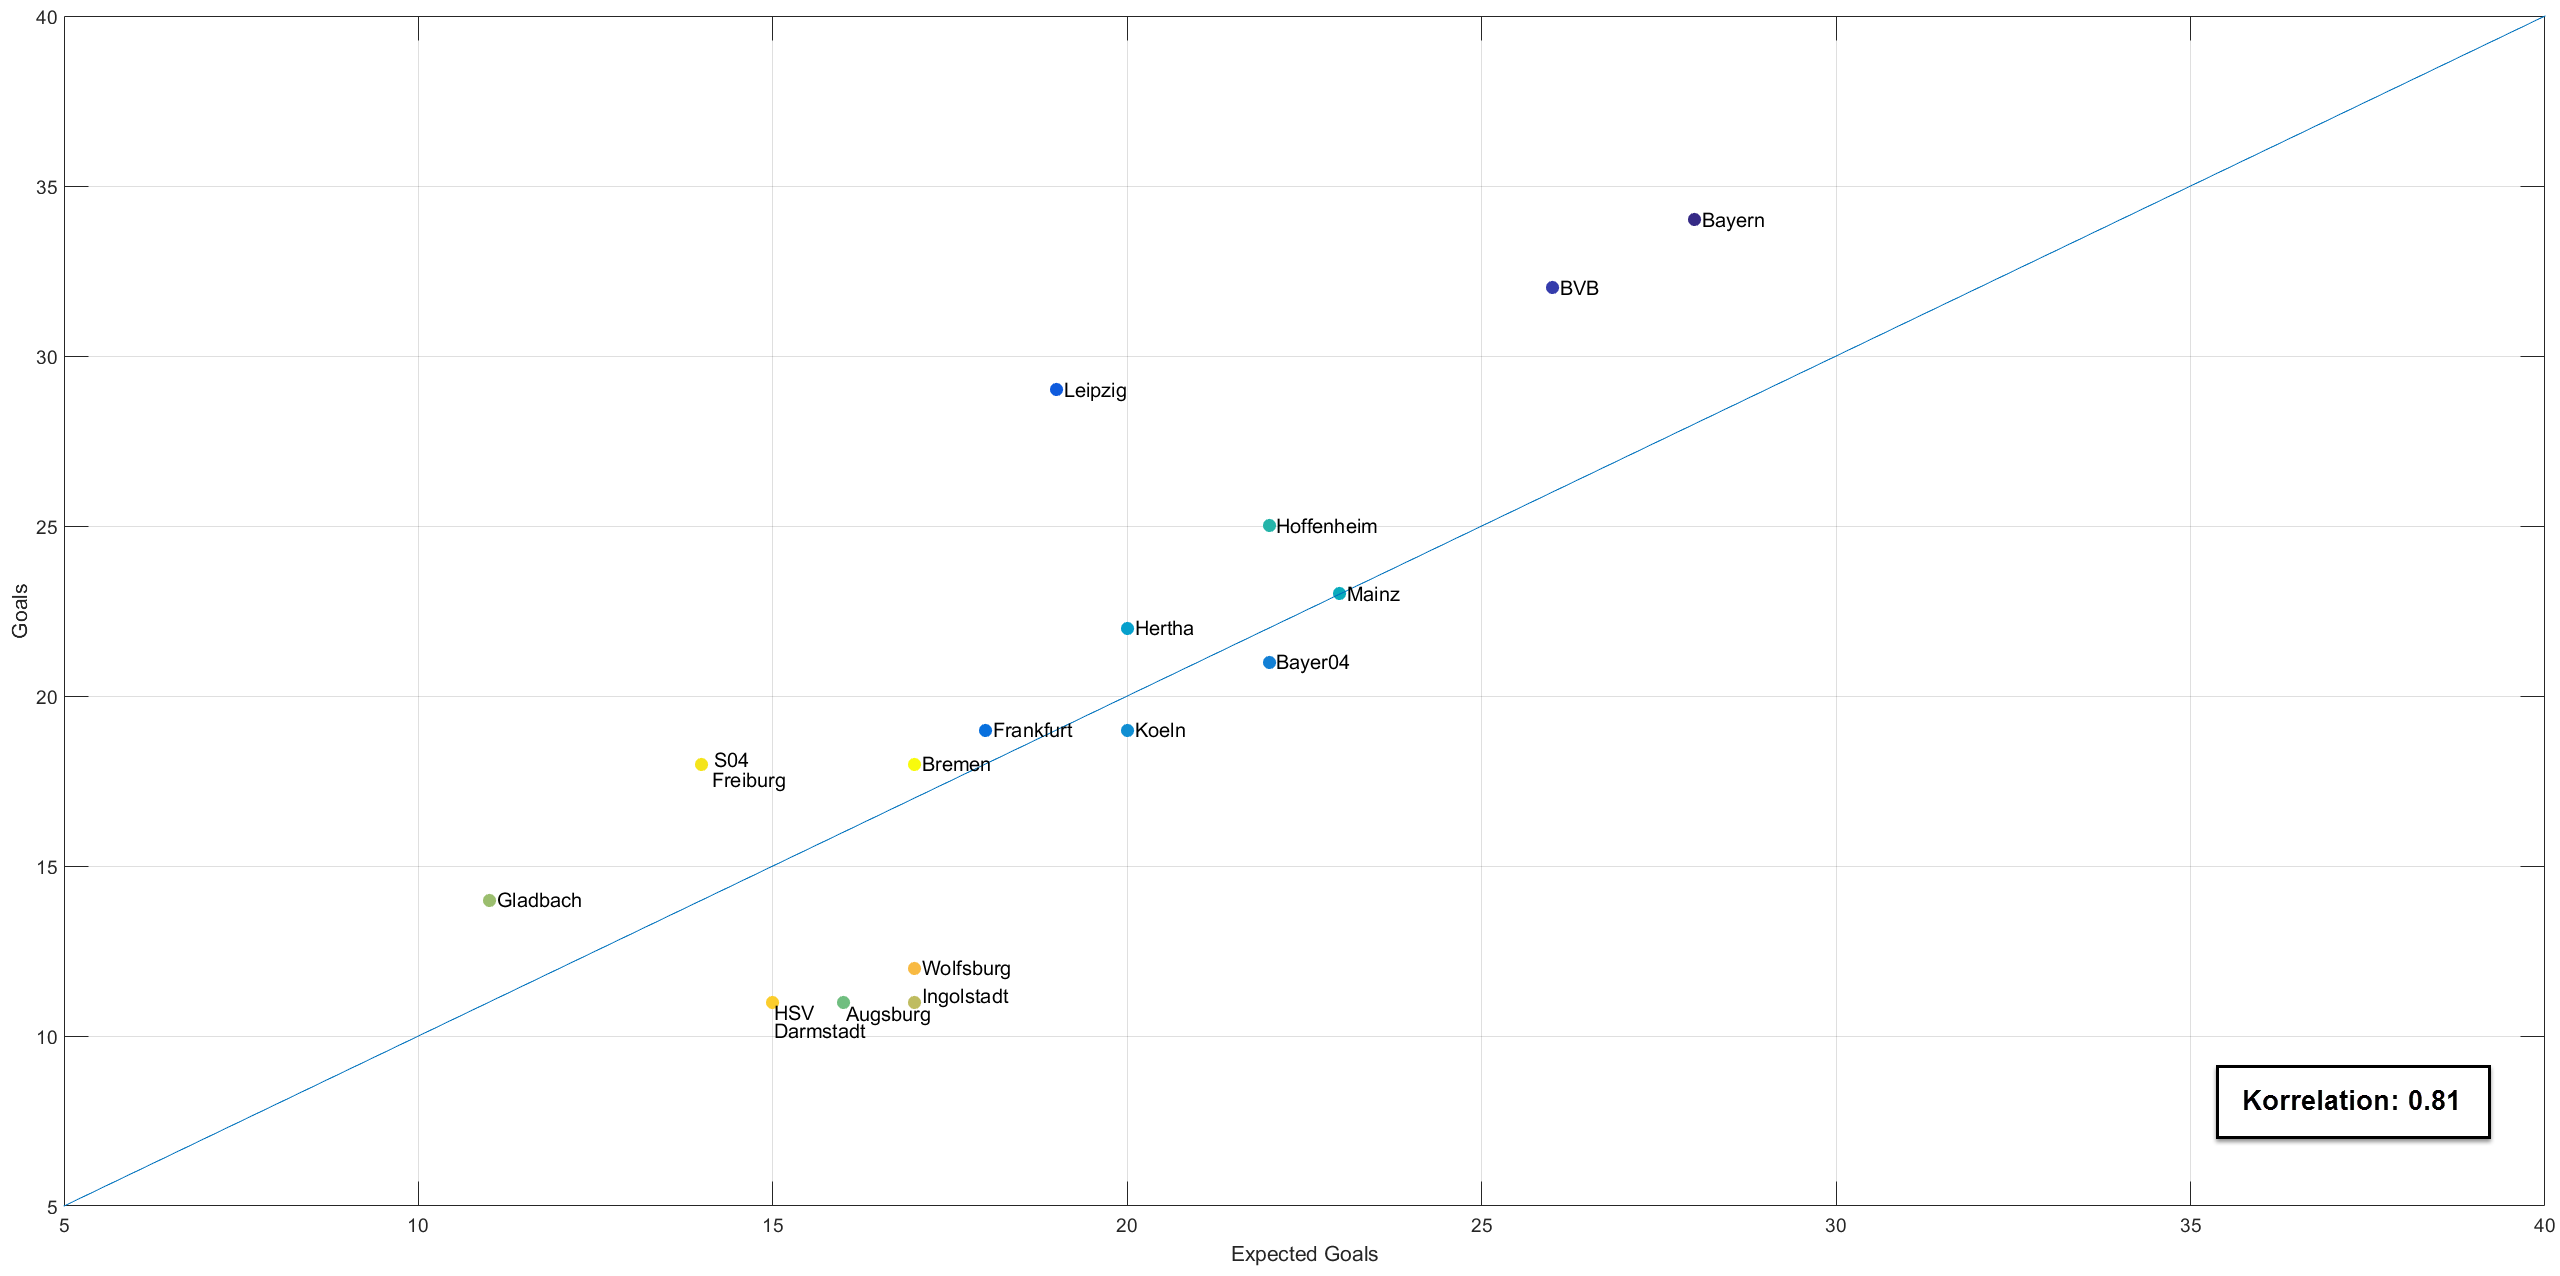
\includegraphics[scale=0.3]{se-wa-jpg/goals_correlation_16_17}
\caption{Evaluation der Tore der Saison 2016/17}
\label{lines}
\end{sidewaysfigure}

\begin{sidewaysfigure}
\centering
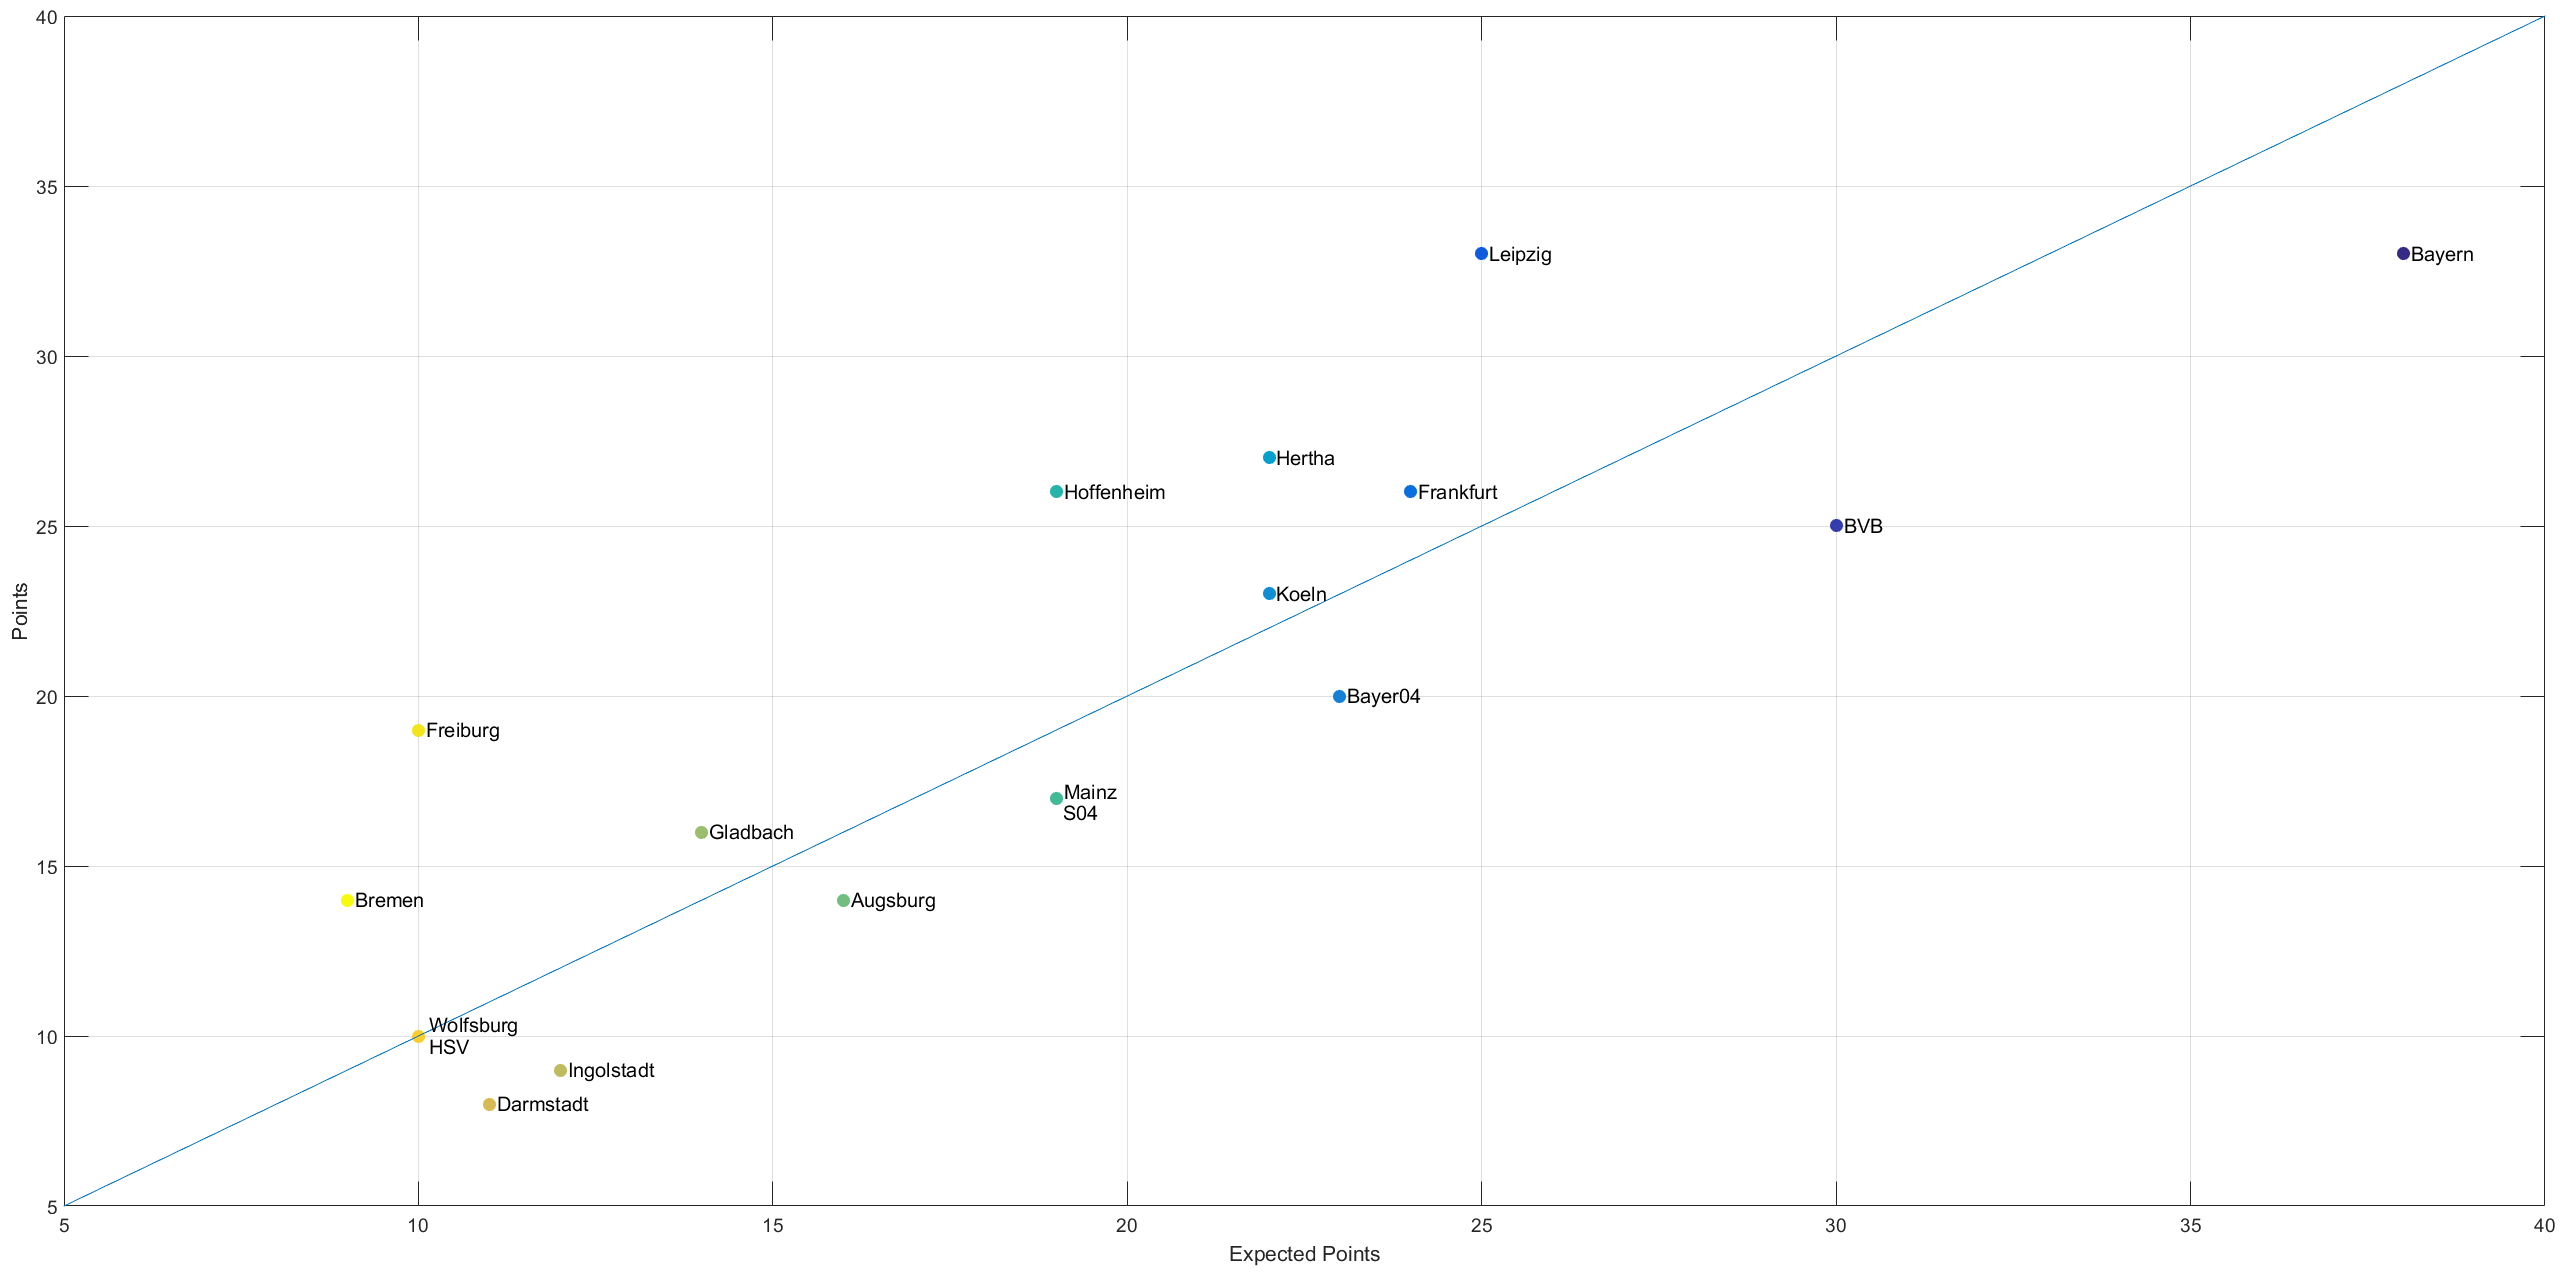
\includegraphics[scale=0.3]{se-wa-jpg/points_correlation_16_17}
\caption{Evaluation der Punkte der Saison 2016/17}
\label{lines}
\end{sidewaysfigure}



